\documentclass[preprint,5p,twocolumn,10pt,sort&compress]{elsarticle}
\newcommand{\upcite}[1]{\textsuperscript{\textsuperscript{ \cite{#1}}}}
%% For including figures, graphicx.sty has been loaded in
%% elsarticle.cls. If you prefer to use the old commands
%% please give \usepackage{epsfig}

%% The amssymb package provides various useful mathematical symbols
\usepackage{amssymb}
%% The amsthm package provides extended theorem environments
 \usepackage{amsthm}
 \usepackage{upgreek}
 \usepackage{graphicx}
  \usepackage{tabularx}
%  \usepackage{multirow}
%\usepackage{xeCJK}
\usepackage{overpic}
\usepackage{caption}
\usepackage{array}
\setlength{\mathindent}{0pt}
\usepackage{booktabs}
\usepackage{epsfig}
\usepackage{textcomp}
\usepackage{subfigure}
\usepackage{natbib}
\usepackage[colorlinks,linkcolor=red,
           				anchorcolor=blue,
            				citecolor=blue]{hyperref}
\usepackage{color,soul}
%% The lineno packages adds line numbers. Start line numbering with
%% \begin{linenumbers}, end it with \end{linenumbers}. Or switch it on

\newcommand{\bfsigma}{{\mbox{\boldmath{$\sigma$}}}}
\newcommand{\bfepsilon}{{\mbox{\boldmath{$\varepsilon$}}}}
\newcommand{\dotbfepsilon}{{\mbox{\boldmath{$\dot\varepsilon$}}}}
\newcommand{\dotbfsigma}{{\mbox{\boldmath{$\dot\sigma$}}}}
\newcommand{\bftau}{{\mbox{\boldmath{$\tau$}}}}
\newcommand{\bfpsi}{{\mbox{\boldmath{$\psi$}}}}
\newcommand{\bfphi}{{\mbox{\boldmath{$\phi$}}}}
\newcommand{\bfalpha}{{\mbox{\boldmath{$\alpha$}}}}
\newcommand{\bfbeta}{{\mbox{\boldmath{$\beta$}}}}
\newcommand{\bfK}{{\bf K}}
\newcommand{\bff}{{\bf f}}
\newcommand{\bfn}{{\bf n}}
\newcommand{\bfm}{{\bf m}}
\newcommand{\bft}{{\bf t}}
\newcommand{\bfu}{{\bf u}}
\newcommand{\bfw}{{\bf w}}
\newcommand{\bfa}{{\bf a}}
\newcommand{\bfb}{{\bf b}}
\newcommand{\bfs}{{\bf s}}
\newcommand{\bfB}{{\bf B}}
\newcommand{\bfD}{{\bf D}}
\newcommand{\bfnabla}{{\mbox{\boldmath{$\nabla$}}}}
\newcommand{\bfDelta}{{\mbox{\boldmath{$\Delta$}}}}
\newcommand{\bfkappa}{{\mbox{\boldmath{$\kappa$}}}}
\newcommand{\bfN}{{\bf N}}
\newcommand{\bfT}{{\bf T}}
\newcommand{\bfG}{{\bf G}}
\newcommand{\bfH}{{\bf H}}
\newcommand{\dd}{{\rm d}}
\newcommand{\degreeC}{{$^\circ$C}}
\newcommand{\marked}[1]{\textcolor{red}{#1}}
\newcommand{\jingyu}[1]{\textcolor{magenta}{#1}}
\renewcommand\figureautorefname{Fig.}
\captionsetup[figure]{labelfont={bf},font={footnotesize},name={Fig.},labelsep=period}

\graphicspath{{figures/}}

\journal{\rm International Journal of Solids and Structures}

\begin{document}


\begin{frontmatter}

%% Title, authors and addresses

%% use the tnoteref command within \title for footnotes;
%% use the tnotetext command for theassociated footnote;
%% use the fnref command within \author or \address for footnotes;
%% use the fntext command for theassociated footnote;
%% use the corref command within \author for corresponding author footnotes;
%% use the cortext command for theassociated footnote;
%% use the ead command for the email address,
%% and the form \ead[url] for the home page:
%% \title{Title\tnoteref{label1}}
%% \tnotetext[label1]{}
%% \author{Name\corref{cor1}\fnref{label2}}
%% \ead{email address}
%% \ead[url]{home page}
%% \fntext[label2]{}
%% \cortext[cor1]{}
%% \address{Address\fnref{label3}}
%% \fntext[label3]{}

\title{Plasticity modeling for a metastable austenitic stainless steel with strain-induced martensitic transformation under cyclic loading conditions}

%% use optional labels to link authors explicitly to addresses:
%% \author[label1,label2]{}
%% \address[label1]{}
%% \address[label2]{}

\author{Cheng LUO}
\author{Wu ZENG}
\author{Jingyu SUN}
\author{Huang YUAN\corref{cor1}}

\address{School of Aerospace Engineering, Tsinghua University, Beijing, China\fnref{label1}}
%\address[label2]{Department of Civil Engineering, Technical University of Darmstadt, Germany\fnref{label2}}
\cortext[cor1]{Corresponding author.}
\ead{yuan.huang@tsinghua.edu.cn}

\begin{abstract}
In the present paper, the strain-induced martensitic transformation and cyclic plasticity model of metastable austenitic steel AISI 348 under multiaxial proportional cyclic loadings were studied. Cyclic loading tests under different stress triaxialities and loading amplitudes were carried out. The variation of martensite content within a loading cycle was investigated and it was observed that the martensite would decrease under certain stress-strain state. On the basis of the Santacreu model, a kinetics model describing the evolution of martensitic transformation under multiaxial cyclic loading was obtained by defining a threshold of equivalent plastic strain for phase transformation. The prediction of martensite content by the model matched well with the experiments. By introducing martensitic transformation strengthening to isotropic hardening, an Ohno-Wang model based cyclic plasticity model of AISI 348 was obtained and the stress-strain response was well described.
\end{abstract}

%\include{debut}
\begin{keyword}
% keywords here, in the form: keyword \sep keyword
Metastable austenitic stainless steel\sep martensitic transformation \sep transformation kinetics  \sep cyclic plasticity \sep multiaxial cyclic loads

% PACS codes here, in the form: \PACS code \sep code
% \PACS
\end{keyword}
\end{frontmatter}

\section{Introduction}
Martensitic transformation is observed in metastable austenitic stainless steels under thermal or mechanical loadings, which has been applied for surface treatment technique to enhance the materials property. The phase transformation of the metastable austenitic stainless steels mainly depends on the temperature as well as chemical composition (\citeauthor{Angel}, \citeyear{Angel}; \citeauthor{Lecroisey1972Martensitic}, \citeyear{Lecroisey1972Martensitic}; \citeauthor{Olson1975Kinetics}, \citeyear{Olson1975Kinetics}; \citeauthor{Hecker1982Effects}, \citeyear{Hecker1982Effects}; \citeauthor{Diani1998Effects}, \citeyear{Diani1998Effects}; \citeauthor{Stringfellow1992A}, \citeyear{Stringfellow1992A})
and can be composed of the stress induced transformation and the strain induced transformation (\citeauthor{Olson1975Kinetics}, \citeyear{Olson1975Kinetics}). During the martensitic transformation, the face-centered cubic (FCC) austenite turns the into body-centered cubic (BCC) martensite. Since austenite is a relatively ductile phase and the martensite possesses a high deformation resistance, that is, the steel is strengthened after the phase transformation (\citeauthor{Santacreu2006Behaviour}, \citeyear{Santacreu2006Behaviour}). In addition, the transformation induces compressive residual stresses and increases the lifetime in the HCF(high cycle fatigue) range of the material. Therefore, the martensitic transformation is served as an important mechanism for manufacturing high-performance parts.

%(\citeauthor{}, \citeyear{})

Many kinetics models for martensitic transformation in the shape memory alloy and TRIP steel were established by studying the correlations between the microstructure and the macroscopic mechanical behavior. The microscopic deformation due to transformation was connected to the macroscopic behavior of shape memory alloys by introducing microregion and mesodomain in alloys (\citeauthor{FISCHER1992A}, \citeyear{FISCHER1992A}). \cite{REISNER19982457} described the strain induced martensitic transformation of austenitic grains on the basis of a criterion proposed by \cite{Fischer1997}. It was found that the grain size, degree of randomness of the austenite's crystallographic lattice orientation with respect to the external load type strongly influenced the stability of the austenite. By combining the crystallographic theory with micromechanics analysis and the internal variable theory, a constitutive model for the forward and reverse martensitic transformation plasticity of single crystal was established in stress space (\citeauthor{YanWY1998A}, \citeyear{YanWY1998A}). A quantitative microstructure-based constitutive model for polycrystalline shape memory alloy was established on the basis of micromechanics, crystallographic theory and transformation criterion (\citeauthor{Song2000Effect}, \citeyear{Song2000Effect}).In addition, it was reported that the interplay of nucleation, growth and orientation distribution of martensite would result in different macroscopic transformation kinematics and kinetics. The influence of mechanical twins on the kinetics of martensitic transformation in TRIP-maraging steel was studied computationally to explain the observations reported by \cite{WANG2014268}. The experimental findings were reproduced well and significant influence of parameters such as parent crystal orientation of austenite island, twinning pattern, and twin density on the overall phenomenon was revealed additionally (\citeauthor{GUPTA2018213}, \citeyear{GUPTA2018213}). However, the macroscopic constitutive model for strain-induced martensitic transformation in austenitic stainless steels, especially under cyclic loadings was rarely discussed.

In past years numerous experimental results on the strain induced martensitic transformation were obtained (\citeauthor{Angel}, \citeyear{Angel}; \citeauthor{Lecroisey1972Martensitic}, \citeyear{Lecroisey1972Martensitic}; \citeauthor{Olson1975Kinetics}, \citeyear{Olson1975Kinetics}; \citeauthor{Hecker1982Effects}, \citeyear{Hecker1982Effects}; \citeauthor{Diani1998Effects}, \citeyear{Diani1998Effects}; \citeauthor{Stringfellow1992A}, \citeyear{Stringfellow1992A}). Transformation kinetics models were proposed and could describe the martensitic transformation under monotonic loadings well. \cite{Olson1975Kinetics} established a function of equivalent plastic strain and temperature to demonstrate the evolution of the martensite content. \cite{Stringfellow1992A} expanded on the Olson and Cohen model by incorporating the effect of the stress triaxiality. \cite{Santacreu2006Behaviour} investigated the austenitic stainless steels for automotive structural parts and improved the Guimar{\~a}es model  (\citeauthor{Guimar1974Temperature}, \citeyear{Guimar1974Temperature}) by coupling the temperature with the maximum  of the martensite content and introducing stress triaxiality. Apart from describing the stress state with stress triaxiality, the lode angle parameter was included by \cite{Beese2011Effect}. For martensitic transformation under cyclic loadings, cyclic strain rate  (\citeauthor{Pegues2017Cyclic}, \citeyear{Pegues2017Cyclic}), strain amplitude  (\citeauthor{Wu2017Mechanical}, \citeyear{Wu2017Mechanical}) as well as accumulated plastic strain  (\citeauthor{Bayerlein1989Plasticity}, \citeyear{Bayerlein1989Plasticity}) were considered in kinetics models. \cite{Smaga2008Deformation} conducted uniaxial cyclic loading tests on three kinds of metastable austenitic steels and modeled the transformation as a function of the accumulated plastic strain and the cumulative strain-energy density. However, the effect of strain amplitudes which is essential for the kinetics model was not taken into account in the  transformation kinetics model under cyclic loadings.Furthermore, the effect of stress triaxiality for multi-axial under cyclic loading was rarely discussed. In addition, most of the known works focused on the influence of temperature and loading history while the plasticity representation which is of importance for the application of the material in industrial design was seldom considered.

\jingyu{The austenitic stainless steel AISI 348 is extensively used in chemical plant constructions in the corrosive environment  (\citeauthor{Nebel2003Cyclic}, \citeyear{Nebel2003Cyclic}). The niobium in AISI 348 improves the corrosive resistance and, however, reduces the stability of the austenitic phase  (\citeauthor{Hahnenberger2014Microstructural}, \citeyear{Hahnenberger2014Microstructural}). The material becomes metastable and can transform into the martensitic phase under mechanical loads (\citeauthor{Smaga2008Deformation}, \citeyear{Smaga2008Deformation}; \citeauthor{Nebel2003Cyclic}, \citeyear{Nebel2003Cyclic}; \citeauthor{Hahnenberger2014Microstructural}, \citeyear{Hahnenberger2014Microstructural}). The martensitic transformation plays an important role in characterizing the mechanical behavior of AISI 348.}

In the present paper, results of multi-axial proportional cyclic loading tests performed in a metastable austenitic stainless steel are reported. Effects of the stress triaxiality and the strain amplitude are clarified  and integrated into the transformation model. A transformation kinetics equation is proposed based on the Santacreu model (\citeauthor{Santacreu2006Behaviour}, \citeyear{Santacreu2006Behaviour}) and the evolution of martensite content is described well in comparing with experimental measurements. A cyclic plasticity model is developed to predict the mechanical behavior of the steel under multi-axial loading and can predict experimental results reasonably. The present work provides a systematic results for plastic deformations with martensitic phase transformation under cyclic loading conditions.


\section{Experiments}

\subsection{Material specification}

\jingyu{The material used in the paper is the stainless steel AISI 348, which was provided by German manufacturer Boehler Edelstahl GmbH. The alloy was delivered in the form of rods with a diameter of 18 mm. The chemical composition of AISI 348 is given in \autoref{Tab:ChemicalComposition}. The rods were solution-treated at 1020\degreeC~ for one hour then cooled to room temperature in water. The metallographic structure of the material was characterized through electron backscatter diffraction (EBSD) analysis. As shown in \autoref{fig:BMmicrostructure}, the initial grains were almost fully austenitic and the average grain size was about $4.5 \rm{\mu m}$.}

% AISI 348 has elastic modulus of $E=$180GPa and yield stress of $\sigma _{0.2}$=270MPa according to the inspection certificate. The martensite start temperature $M_{\rm s}$ estimated using the empirical Eichelman and Hull formula (\citeauthor{Eichelman}, \citeyear{Eichelman}) is close to -241\degreeC. 

% From known experimental observations (\citeauthor{Smaga2008Deformation}, \citeyear{Smaga2008Deformation}; \citeauthor{Nebel2003Cyclic}, \citeyear{Nebel2003Cyclic}; \citeauthor{Hahnenberger2014Microstructural}, \citeyear{Hahnenberger2014Microstructural}) the austenite AISI 348 can transfer to martensite at different extent of deformations.

\begin{table}[!ht]
  \centering
  \caption{\jingyu{Chemical compositions of AISI 348 (wt. \%)}}
    \begin{tabular}{llll}
    \toprule
    Element & wt. \% & Element & wt. \% \\
    \midrule
    Cr    & 17.16  & Ni    & 10.46 \\
    C     & 0.07   & Mn    & 1.93 \\
    Mo    & 0.27   & Co    & 0.07 \\
    Nb    & 0.40   & Ta    & 0.002 \\
    Si    & 0.39   & P     & 0.021 \\
    S     & $\leq$0.003    & Fe     & Balance \\
    \bottomrule
    \end{tabular}%
  \label{Tab:ChemicalComposition}
\end{table}

\begin{figure}[!htp]
  \begin{center}
  
\includegraphics[width=8cm]{BMmicrostructure.png}
  \caption{Microstructure of as-received AISI 348 stainless steel characterized by EBSD. The initial microstructure was almost fully austenitic and the average grain size was $4.5 \rm{\mu m}$.}
  \label{fig:BMmicrostructure}
  \end{center}
\end{figure}

%\begin{table}[!h]
%	\begin{center}
%	\caption{Initial mechanical properties of the stainless steel AISI 348}
%    \label{tab:Mechanical Properties}
%		\begin{tabular}{ c c c c }  \hline %means horizon line
%		Elastic modulus & Yield Stress  & Tensile Strength & Fracture Strain \\  \hline
%		180GPa&400MPa&605MPa&53$\%$ \\  \hline
%		\end{tabular}
%	\end{center}
%\end{table}

\subsection{Specimens}

\jingyu{Cylindrical and tubular specimens were machined for uniaxial and biaxial test, respectively. The dimension of the cylindrical specimen is shown in \autoref{Fig:Specimen}(a), the gauge length of the cylindrical specimen is equal to 20 mm and the diameter of the gauge section is 10 mm. \autoref{Fig:Specimen}(b) shows the gauge length of the tubular specimen is equal to 30 mm and the inner and outer diameters of the gauge section are 10 mm and 12.5 mm, respectively. All specimens were polished to obtain smooth surface.}

	\begin{figure}[!htp]
    \centering
    \begin{overpic}[width=8.0cm]{SS348_Solid.pdf}
        \put(90,20){\fcolorbox{white}{white}{(a)}}
    \end{overpic}
    \begin{overpic}[width=8.0cm]{SS348_Tubular.pdf}
        \put(90,20){\fcolorbox{white}{white}{(b)}}
    \end{overpic}
    \caption{\jingyu{Dimensions of the specimen: (a) cylindrical for uni-axial tests and (b) tubular for biaxial tests.}}
    \label{Fig:Specimen}
\end{figure}

\subsection{Tests procedure}

\jingyu{All tests were conducted on a servo hydraulic tension-torsion test machine under strain controlled at room temperature. An uniaxial extensometer with gauge length of 10 mm was used in the tension-compression test. In the biaxial test, the axial and shear strain were measured by an tension-torsional extensometer with gauge length of 25 mm. Fully reversed strain-controlled cyclic experiments were carried out for the 4 types of loading, summarized in detail in \autoref{Tab:LoadPath}. The loading paths contains tension-compression, torsion, proportional loading and non-proportional loading. The triangle-shaped strain waveforms were used to keep the strain rate constant in all tests. }

\jingyu{Equivalent mechanical strain, $\varepsilon_{\mathrm{eq}}=\sqrt{\varepsilon^{2}+\gamma^{2} / 3}$, is calculated in analogy to the von Mises stress. The loading ratios for all tests were the same as $R_{\varepsilon }=-1$. The equivalent strain amplitudes were shown in \autoref{Tab:test_matrix}. The cyclic loading tests were kept running until the measured MC reached a certain value (50\%-ferrite) or until the specimens failure.}

\begin{figure}[!htp]
  \begin{center}
  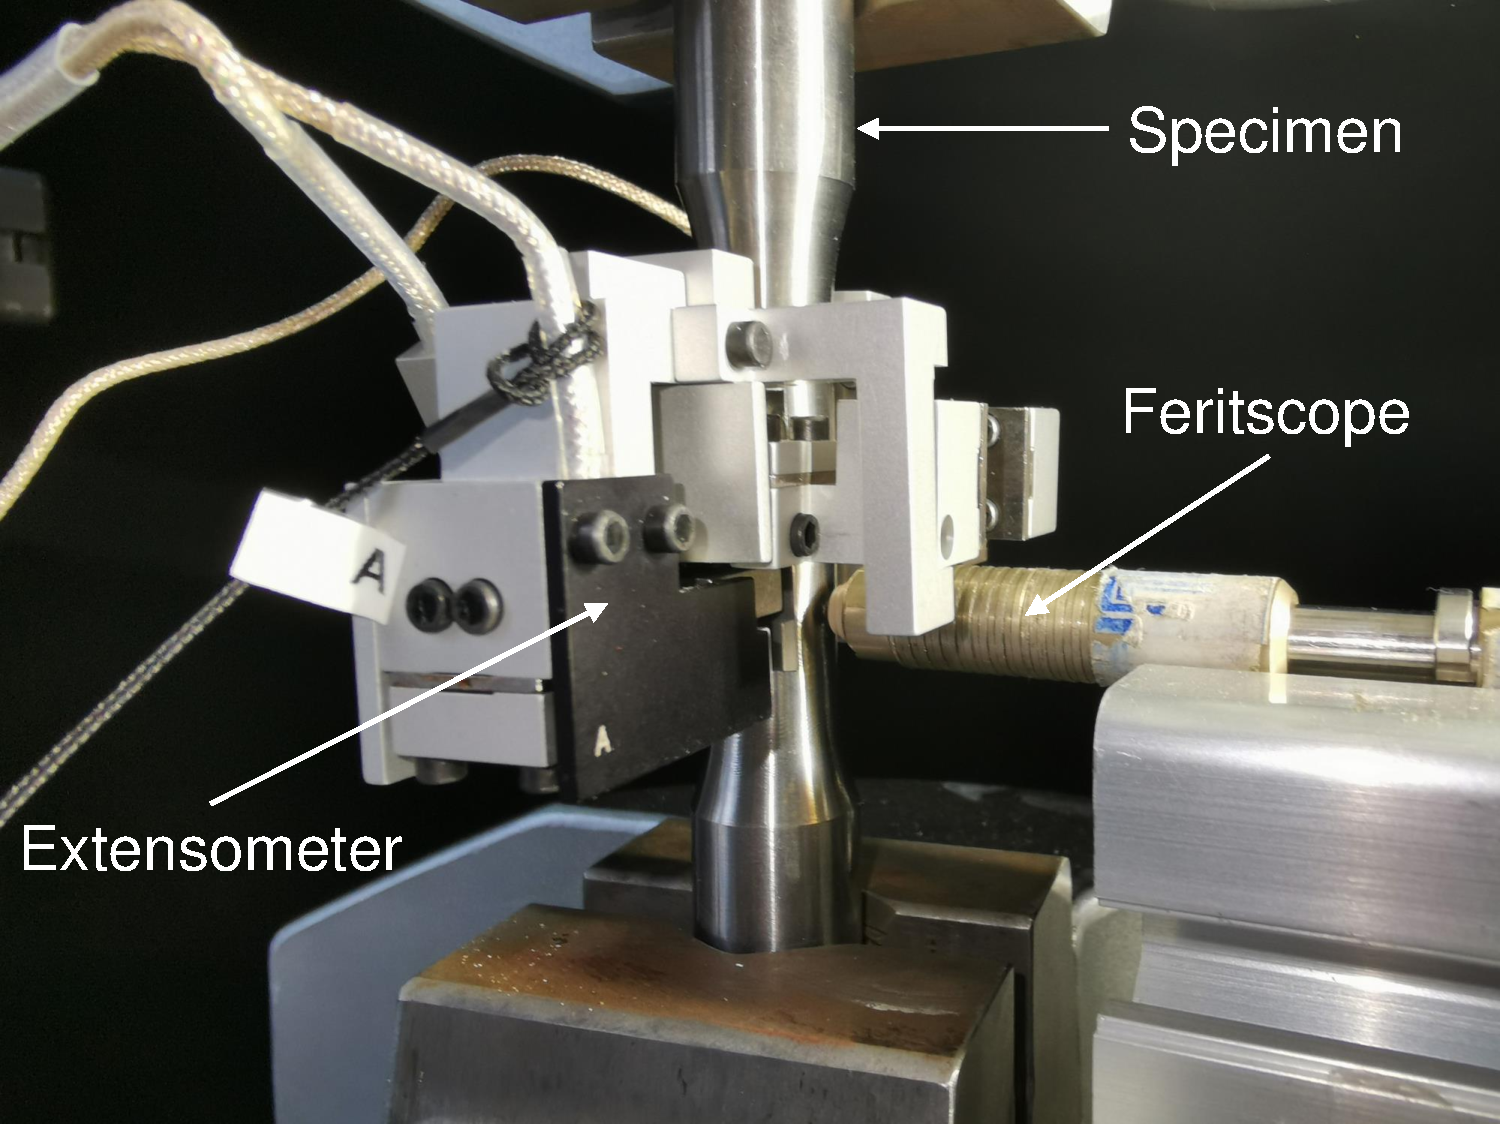
\includegraphics[width=8cm]{TestSetup.pdf}
  \caption{\jingyu{Cyclic tension-torsional test with the extensometer and the Feritscope.}}
  \label{fig:Testsetting}
  \end{center}
\end{figure}

\begin{table*}[!ht]
  \centering
  \caption{\jingyu{Loading paths of cyclic tests.}}
    \begin{tabular}{p{2.0cm}p{4.0cm}p{4cm}p{4cm}}
    \toprule
    Symbol & Type of loading & Loading wave & Strain path  \\
    \midrule
    TC     & tension-compression  & \begin{minipage}{0.1\textwidth}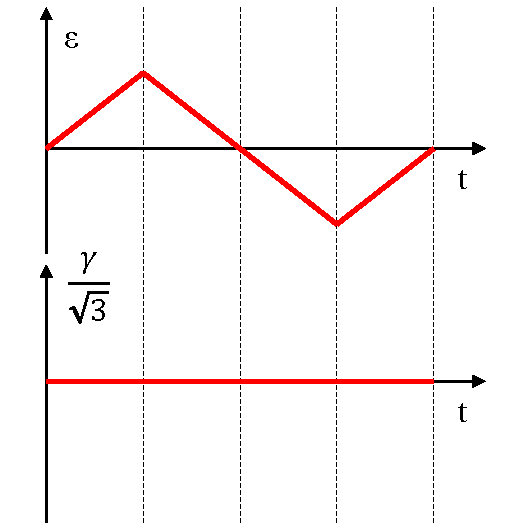
\includegraphics[width=3cm]{load_path_1_time.pdf}\end{minipage}  & \begin{minipage}{0.1\textwidth}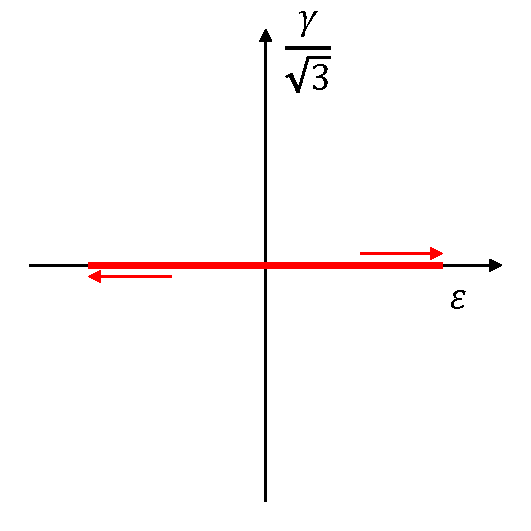
\includegraphics[width=3cm]{load_path_1.pdf}\end{minipage} \\
	\midrule
    TOR    & torsion  & \begin{minipage}{0.1\textwidth}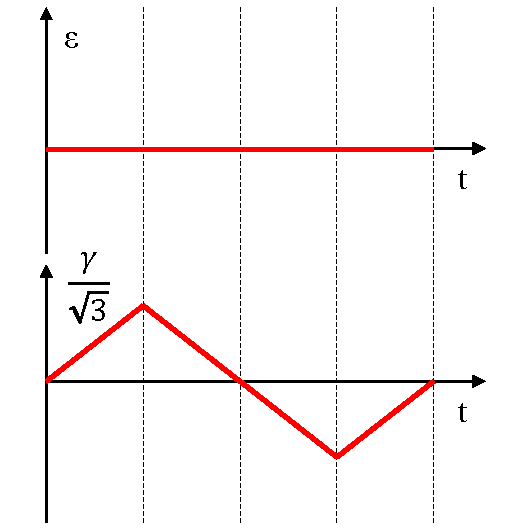
\includegraphics[width=3cm]{load_path_2_time.pdf}\end{minipage}  & \begin{minipage}{0.1\textwidth}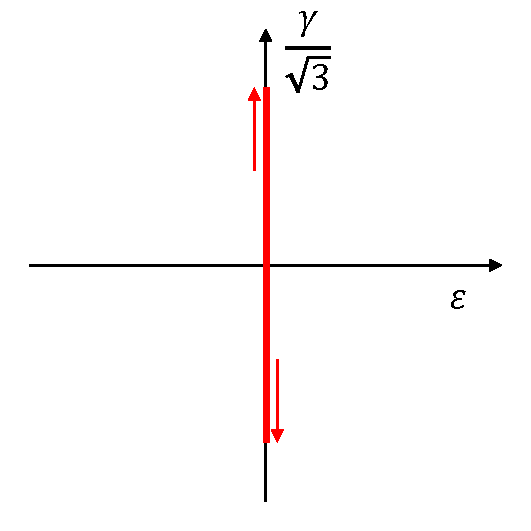
\includegraphics[width=3cm]{load_path_2.pdf}\end{minipage} \\
	\midrule
    PRO    & proportional  & \begin{minipage}{0.1\textwidth}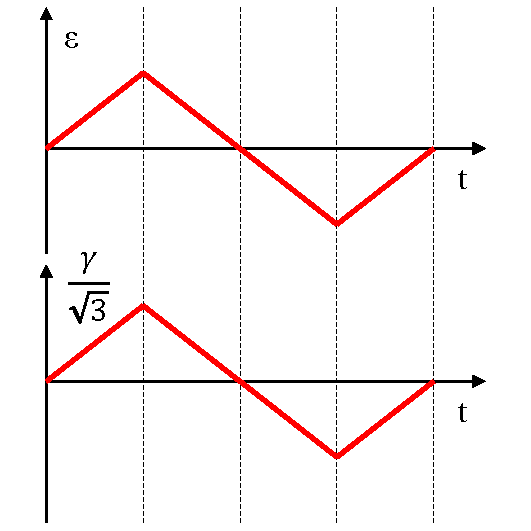
\includegraphics[width=3cm]{load_path_3_time.pdf}\end{minipage}  & \begin{minipage}{0.1\textwidth}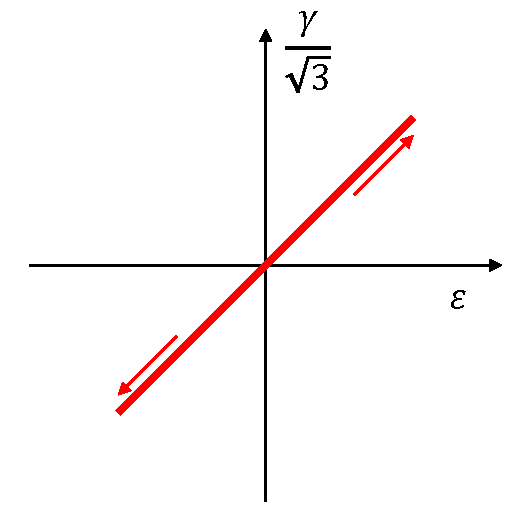
\includegraphics[width=3cm]{load_path_3.pdf}\end{minipage} \\
	\midrule
    NPR    & non-proportional  & \begin{minipage}{0.1\textwidth}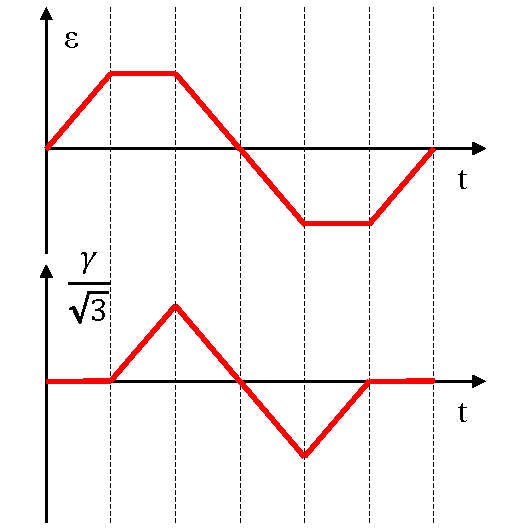
\includegraphics[width=3cm]{load_path_4_time.pdf}\end{minipage}  & \begin{minipage}{0.1\textwidth}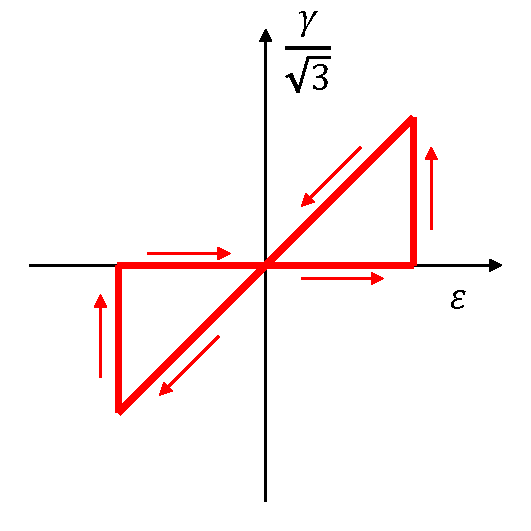
\includegraphics[width=3cm]{load_path_4.pdf}\end{minipage} \\
    \bottomrule
    \end{tabular}%
  \label{Tab:LoadPath}%
\end{table*}%

\begin{table}[!ht]
  \centering
  \caption{\jingyu{Experimental conditions of the tests.}}
    \begin{tabular}{p{2.0cm}p{1.0cm}<{\centering}p{1cm}<{\centering}p{1cm}<{\centering}p{1.5cm}<{\centering}}
    \toprule
    Strain path & $\Delta \varepsilon _{\rm{eq}}/2$ & $\Delta \varepsilon$/2 & $\Delta \gamma $/2 &$\dot \varepsilon _{\rm{eq}}$ \\
        & [\%]  & [\%] & [\%] & [s$^{-1}$] \\
    \midrule
    TC    & 1.00  & 1.00 & 1.73  & $8\times 10^{-3}$ \\
          & 0.80  & 0.80 & 1.38  & $8\times 10^{-3}$ \\
          & 0.50  & 0.50 & 0.87  & $8\times 10^{-3}$ \\
    \midrule      
    TOR   & 1.00  & 1.00 & 1.73  & $8\times 10^{-3}$ \\
          & 0.80  & 0.80 & 1.38  & $8\times 10^{-3}$ \\
          & 0.50  & 0.50 & 0.87  & $8\times 10^{-3}$ \\
    \midrule
    PRO   & 1.00  & 1.00 & 1.73  & $8\times 10^{-3}$ \\
   	\midrule
    NPR   & 1.00  & 1.00 & 1.73  & $8\times 10^{-3}$ \\
    \bottomrule
    \end{tabular}%
  \label{Tab:test_matrix}%
\end{table}%

\jingyu{The martensitic phase content in the specimen was measured in situ using a ferritescope 'Fischer FERITSCOPE FMP30'. The ferritescope measures according to the magnetic induction method. A magnetic field generated by the probe interacted with the magnetic volume fraction of the specimen. The change of the magnetic field induces a voltage proportional to the magnetic fraction in a measuring coil. If the martensitic phase is the only magnetic content in the specimen, then its volume fraction is linearly proportional to the output signal. Period to the test, the ferritescope was calibrated with the calibration samples. The position between the probe and the specimen influences the measuring results. Thus, during the tests, the measurement probe of the feritscope was perpendicular to the surface of the specimen, as presented in \autoref{fig:Testsetting}. The contact force between the probe and the specimen was kept constant during the experiments.}

\jingyu{The martensitic phase transformation is sensitive to the temperature (need some refs). \cite{Smaga2008Deformation} kept the loading frequency at 0.2Hz and the temperature variation of the specimens was below 20\degreeC. In the study, the strain rates were below $8\times 10^{-3}$, in order to keep the temperature of the specimen below 20\degreeC.}

% It is known that the Villari effect (Inverse magnetostrictive effect) affects the measurement of martensite in stainless steels, which refers to the fact that the materials have a change of magnetic susceptibility when subjected to mechanical stressing. 
The measurement range of the Feritscope is 0$\sim$80\% Fe. The reading of the Feritscope was designed for the ferrite instead of the martensite, so calibration and amendment were required for the actual martensite content. The conversion coefficient for the readings of Feritscope to the actual MC was recommended  by \cite {Talonen2004} as 1.7.

\jingyu{On the other side, due to the inverse magnetostriction, the magnetization of ferromagnetic materials changes with mechanical loadings imposed to the material, the so-called Villari effect. The Villari effect may affect the measured magnetic intensity and be explained by the mechanically induced rotation of domains of uniform polarization within a ferromagnetic material. Generally, mechanical loading decreases the magnetic field intensity. Thus, the measured results under different loading conditions cannot indicate the actual value of the ferrite fraction. To eliminate the Villari effect, the applied mechanical loads on the specimens have to be removed before the measurement. In the study, the stress was unloaded to zero and the stress-free condition was kept for 10 seconds before the data recorded.}

% The contact condition on the head of the probe has minor influence on readings. The probe should be in contact with the surface of the specimens during tests. To overcome this problem, an aluminum holder was fabricated to fix the measurement probe and rubber bands were used to keep the contact pressure constant.

After the cyclic loading tests, the specimens were sectioned and polished for metallographic analysis. In order to remove the interference of the martensite content which might newly grow during the mechanical grinding and polishing, electrochemical polishing was conducted before XRD (X-Ray diffraction) observations.

%Considering the geometry effect additionally, XRD method was used to confirm the conversion coefficient.

%\subsection{Microstructure investigation}
%
%Gauge sections were cut off from the fatigue specimens and mounted and metallographically prepared using standard metallographic procedures.
%%The specimens were then observed through an optical microscope and the grain size together with area fraction of $\alpha ^{'}$ phase were analysed digitally.
%
%XRD analysis was conducted on the specimens using a X350A with Cr k$\alpha$ x-rays with a 2$\theta$ range of 132–125$^{\circ}$ and 168–144$^{\circ}$and a scan rate of 0.1$^{\circ}$ s$^{-1}$. The X-ray tube operating parameters were 25 kV and 5 mA. Five specimens which contained different amount of strain-induced martensite from 0$\%$ to 52$\%$ ($\%$-ferrite) were selected for XRD analysis. The MCs of 5 cyclic loaded specimens were obtained by measuring the austenite phase in the material through XRD analysis. The comparison of martensite contents measured respectively by Feritscope and XRD method is demonstrated in Fig. \ref{fig:XRDandferitscope}. A linear correlation is established to convert the Feritscope readings to actual martensite content.
%
%\begin{figure}[!h]
%  \begin{center}
%  \includegraphics[width=8cm]{XRDandferitscope.pdf}
%  \caption{Comparison of martensite contents measured by Feritscope and XRD}
%  \label{fig:XRDandferitscope}
%  \end{center}
%\end{figure}
%
%As shown in Fig. \ref{fig:XRDandferitscope}, the actual value of the martensite content could be obtained by multiplying with a conversion coefficient of 1.69 on the readings of Feritscope. The martensite contents displayed in the following are all converted to the actual values.

%\begin{figure}[!h]
%  \begin{center}
%  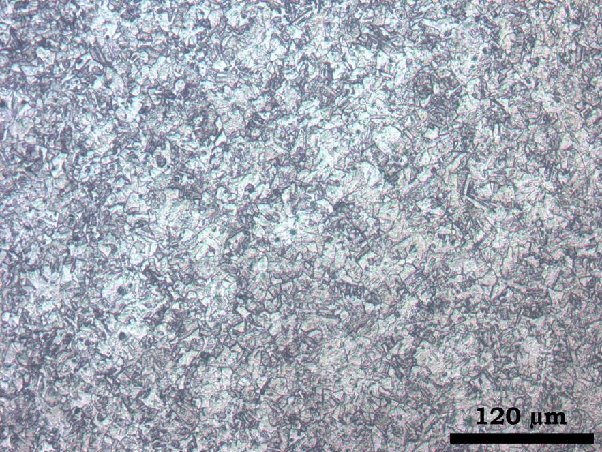
\includegraphics[width=8cm]{microstructureOM.pdf}
%  \caption{Microstructure of the martensitic transformed specimen through OM}
%  \label{fig:microstructureOM}
%  \end{center}
%\end{figure}


\section{Experimental Results and Discussion}

\subsection{Martensite development from cyclic loading}

The martensite content (MC) as a function of the cycle number is plotted in Fig. \ref{fig:total2}.  In the figure, only the values after loading cycles are summarized and three different strain ranges are considered with two different loading paths, axial tension/compression as well as pure torsion. Variations of  MC are discussed in next section. The results reveal that the accumulated martensitic content development is sensitive to the strain range, but independent of stress triaxiality explicitly. It is shown that the growth rate of MC accelerates first and then slows down along the number of cycles. In addition, the material experiences cyclic softening at the beginning and is distinct in secondary cyclic hardening afterwards. The evolution of equivalent stress amplitudes versus the number of cycles during the cyclic loading tests is displayed in Fig. \ref{fig:total1} and confirms the known sensitivity to the loading configuration.

To study the specimen scattering, three specimens were tested for $\varepsilon_{\rm a}=0.8\%$, termed as Axial 0.8\%, Axial 0.8\% Test1, Axial 0.8\% Test2 in the figure, respectively. A larger deviation is found near material fatigue failure.  It is known that the martensitic phase will accelerate damage process and the different MC values make unstable damage more obvious. The scattering of the specimens is limited within a small regime and does not affect the main conclusions.

\begin{figure}[!h]
  \begin{center}
  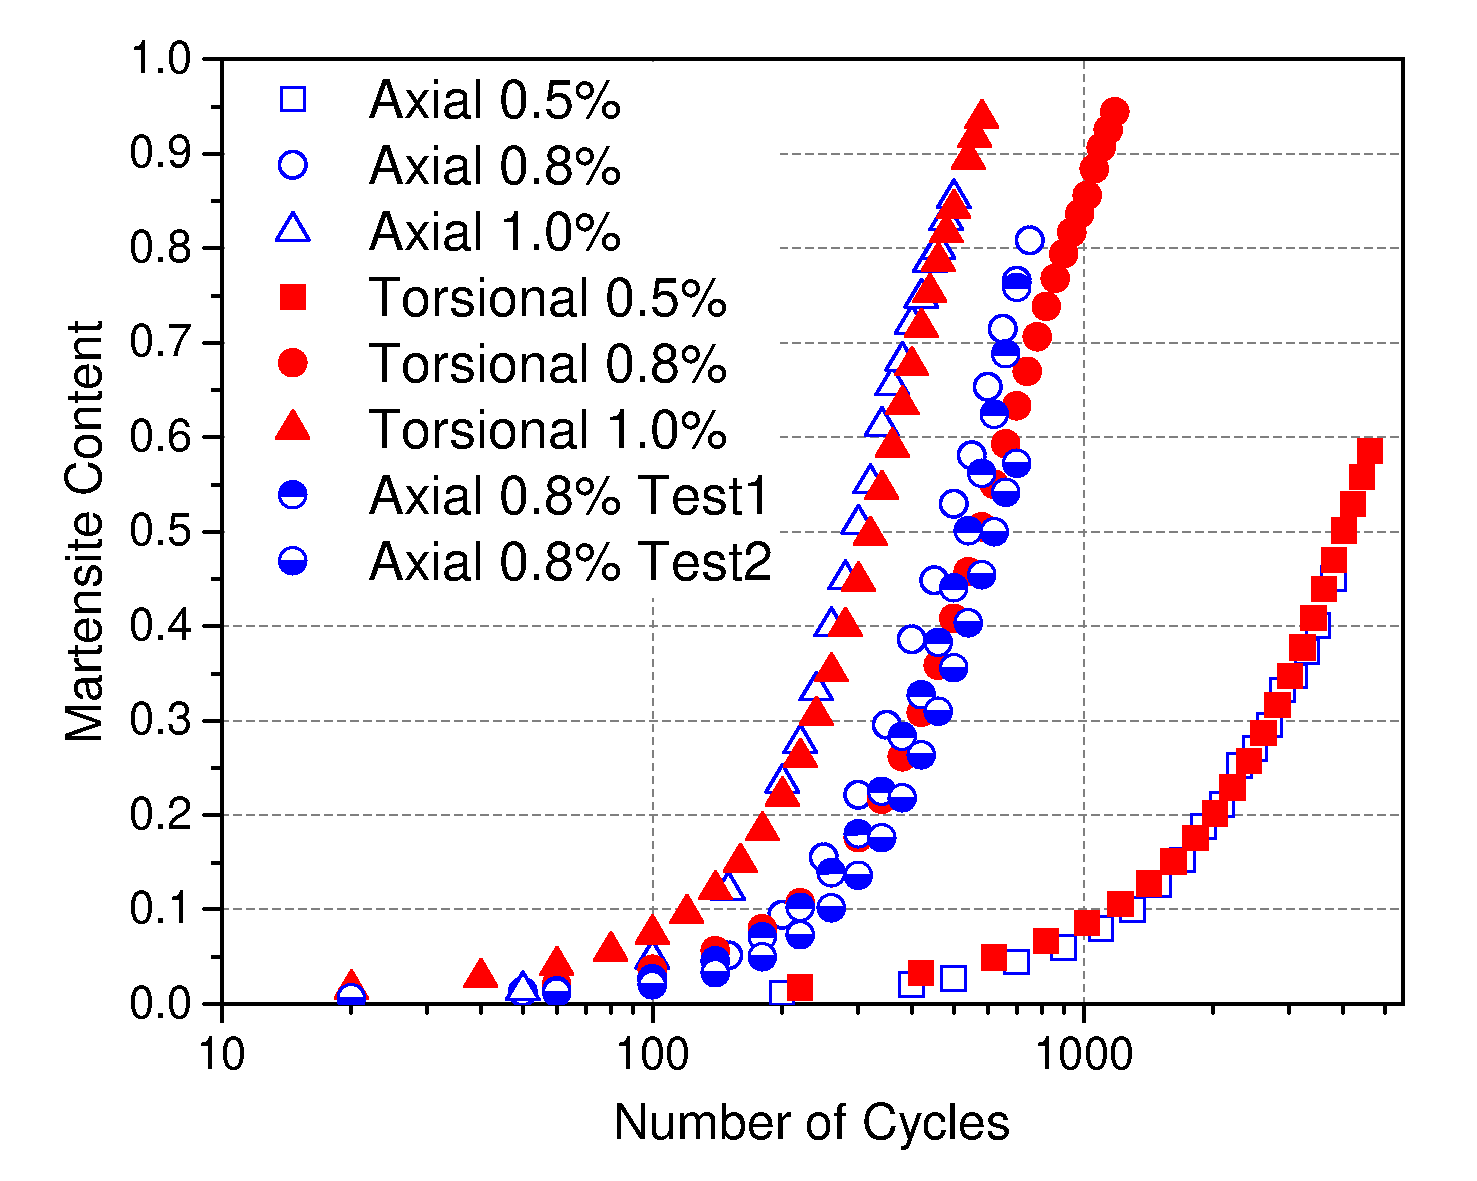
\includegraphics[width=8cm]{total2.pdf}
  \caption{Evolution of MC along the number of cycles in strain range controlled fatigue tests. It reveals that the martensitic content development is sensitive to the strain range, but independent of stress triaxiality explicitly.}
  \label{fig:total2}
  \end{center}
\end{figure}

\begin{figure}[!htb]
  \begin{center}
  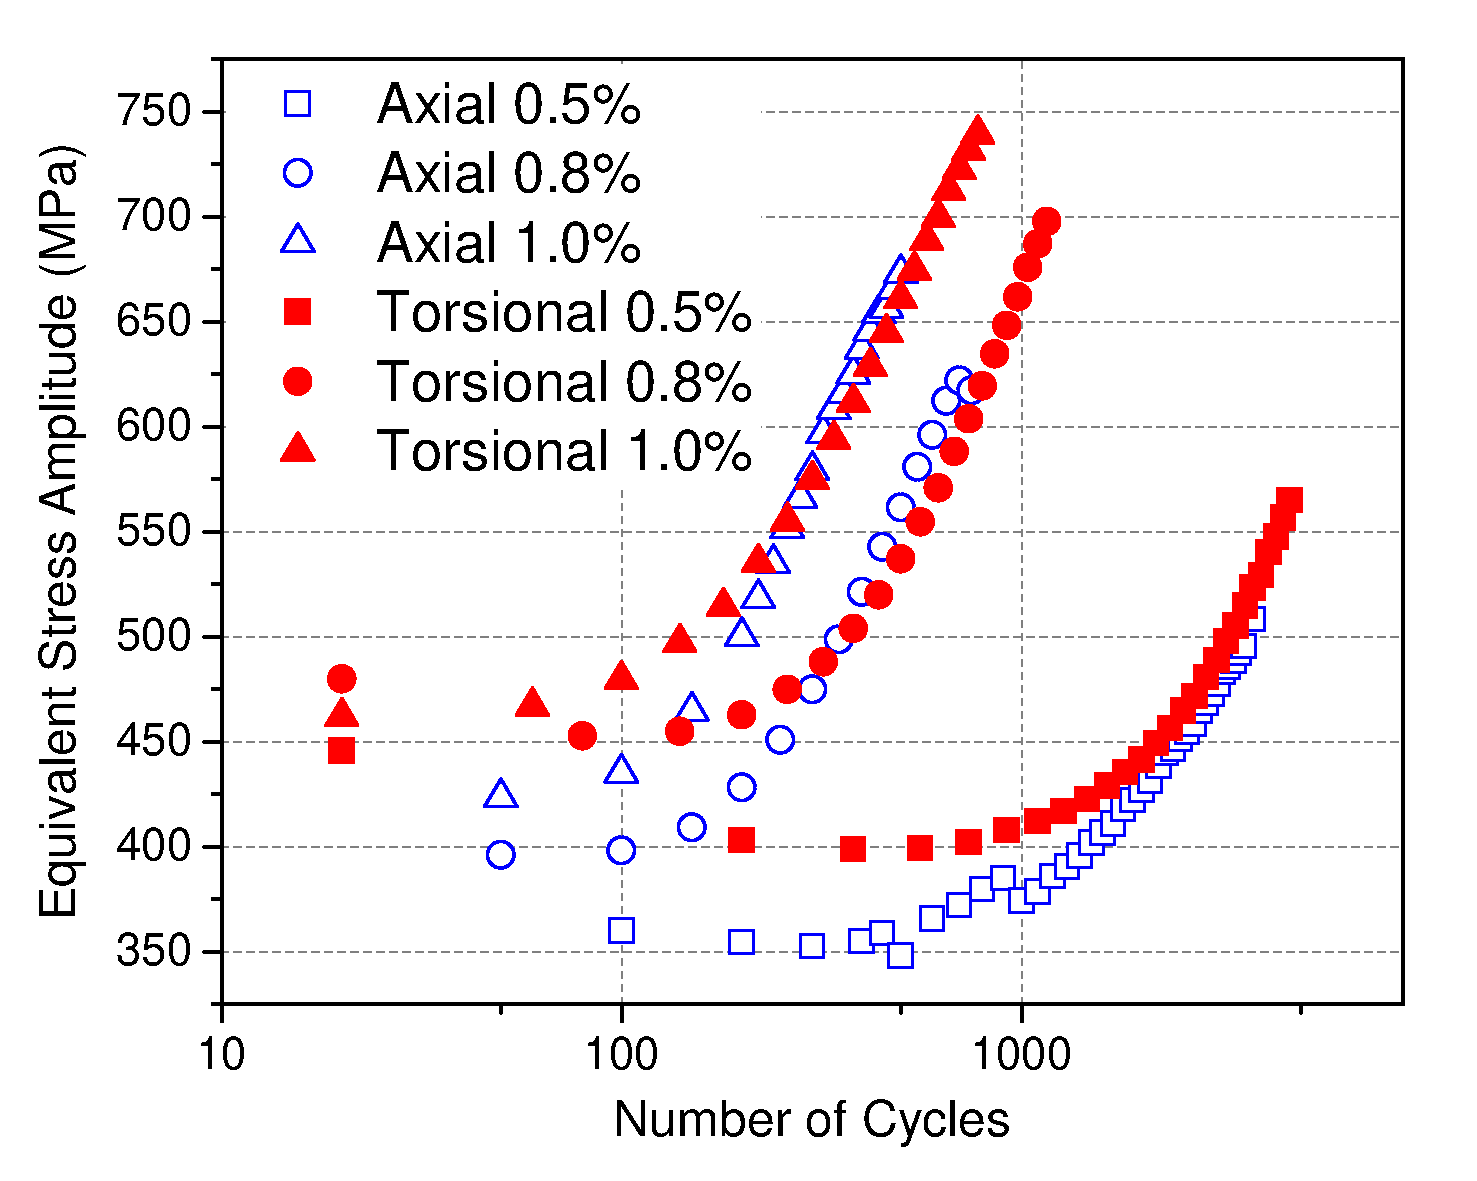
\includegraphics[width=8cm]{total1.pdf}
  \caption{Equivalent stress amplitudes versus the number of cycles in strain range controlled fatigue tests. The material shows cyclic softening at the beginning and is distinct in secondary cyclic hardening afterwards. }
  \label{fig:total1}
  \end{center}
\end{figure}

The cyclic softening was considered to be the result of the rearrangement of the dislocation structure which tends to promote the greater dislocation mobility. Similar cyclic secondary hardening was reported for the steel AISI304 and correlated to the increase of  MC (\citeauthor{Pegues2017Cyclic}, \citeyear{Pegues2017Cyclic}). Cyclic secondary hardening  was defined as the difference between the current stress amplitude and the minimum stress amplitude at the end of cyclic softening. As indicated in Fig. \ref{fig:SecondaryHardening}, the cyclic secondary hardening  increases linearly with  MC. Therefore, it is reasonable to suggest that the martensitic transformation has strong influence on the hardening behavior in AISI 348.

\begin{figure}[!h]
  \begin{center}
  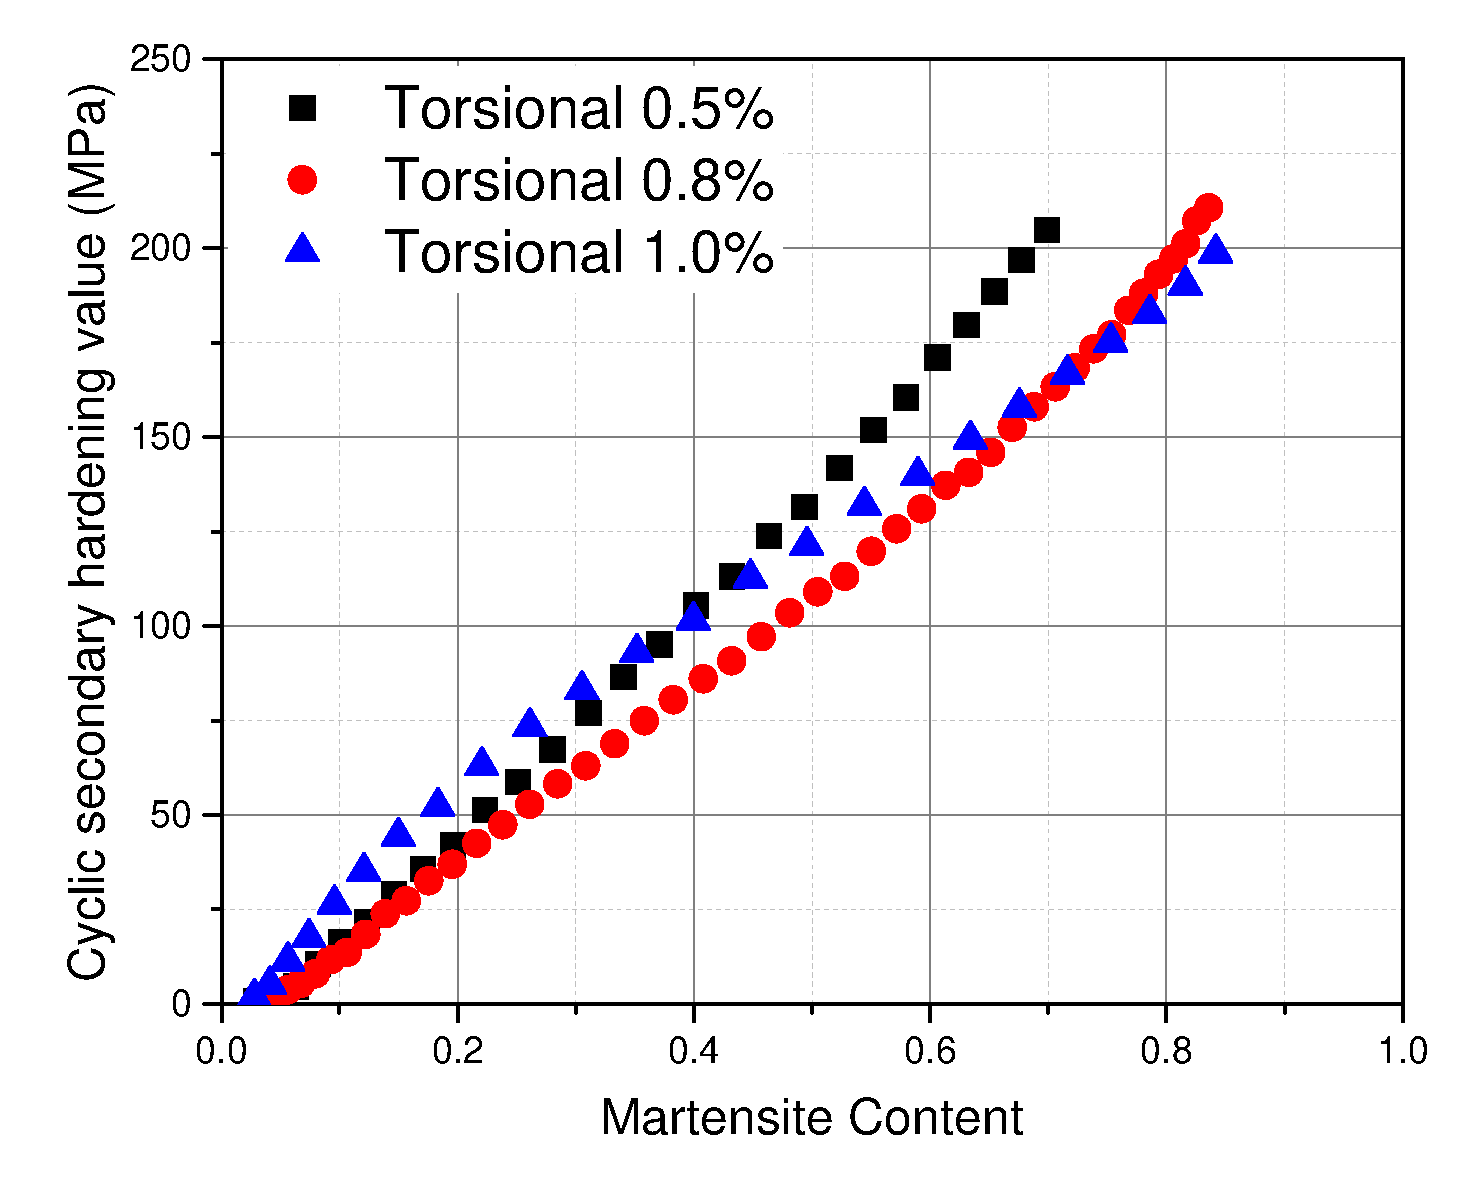
\includegraphics[width=8cm]{SecondaryHardening.pdf}
  \caption{Cyclic secondary hardening defined by \cite{Pegues2017Cyclic} versus the martensite content. The martensitic transformation has strong influence on the hardening behavior.}
  \label{fig:SecondaryHardening}
  \end{center}
\end{figure}

\subsection{Variations of martensite content within a loading cycle}

The martensitic phase transformation depends on stress state and plastic deformations. Due to the Villari effect, MC values were measured at end of each loading cycles in stress-free state. It is interesting to study variations of the martensitic phase within a loading cycle, which consists of loading, unloading as well as reversal loading. In the present work, a loading cycle is decomposed into four segments: loading A-B, unloading B-C, compressive loading C-D and compressive unloading (D-A), as in Fig. \ref{fig:PointDefinition}. Points A, B, C, D are zero-strain ($\varepsilon=0$) points and corner points of the cycle respectively.  In each segment several measure points can be inserted by releasing the applied stress linearly elastically. For example, four additional unloads were added at $\varepsilon=0.25\%,0.50\%,0.75\%,1.0\%$ in the loading segment (A-B) in the 150th cycle with $\varepsilon_{\rm a}=1.0\%$. As results, the loading A-B was realized in 4 sub-steps and the martensite contents corresponding to these 4 points were measured respectively. Since unloading does not cause the phase transformation, the martensitic content is not influenced by the unloadings.

\begin{figure}[!h]
  \begin{center}
  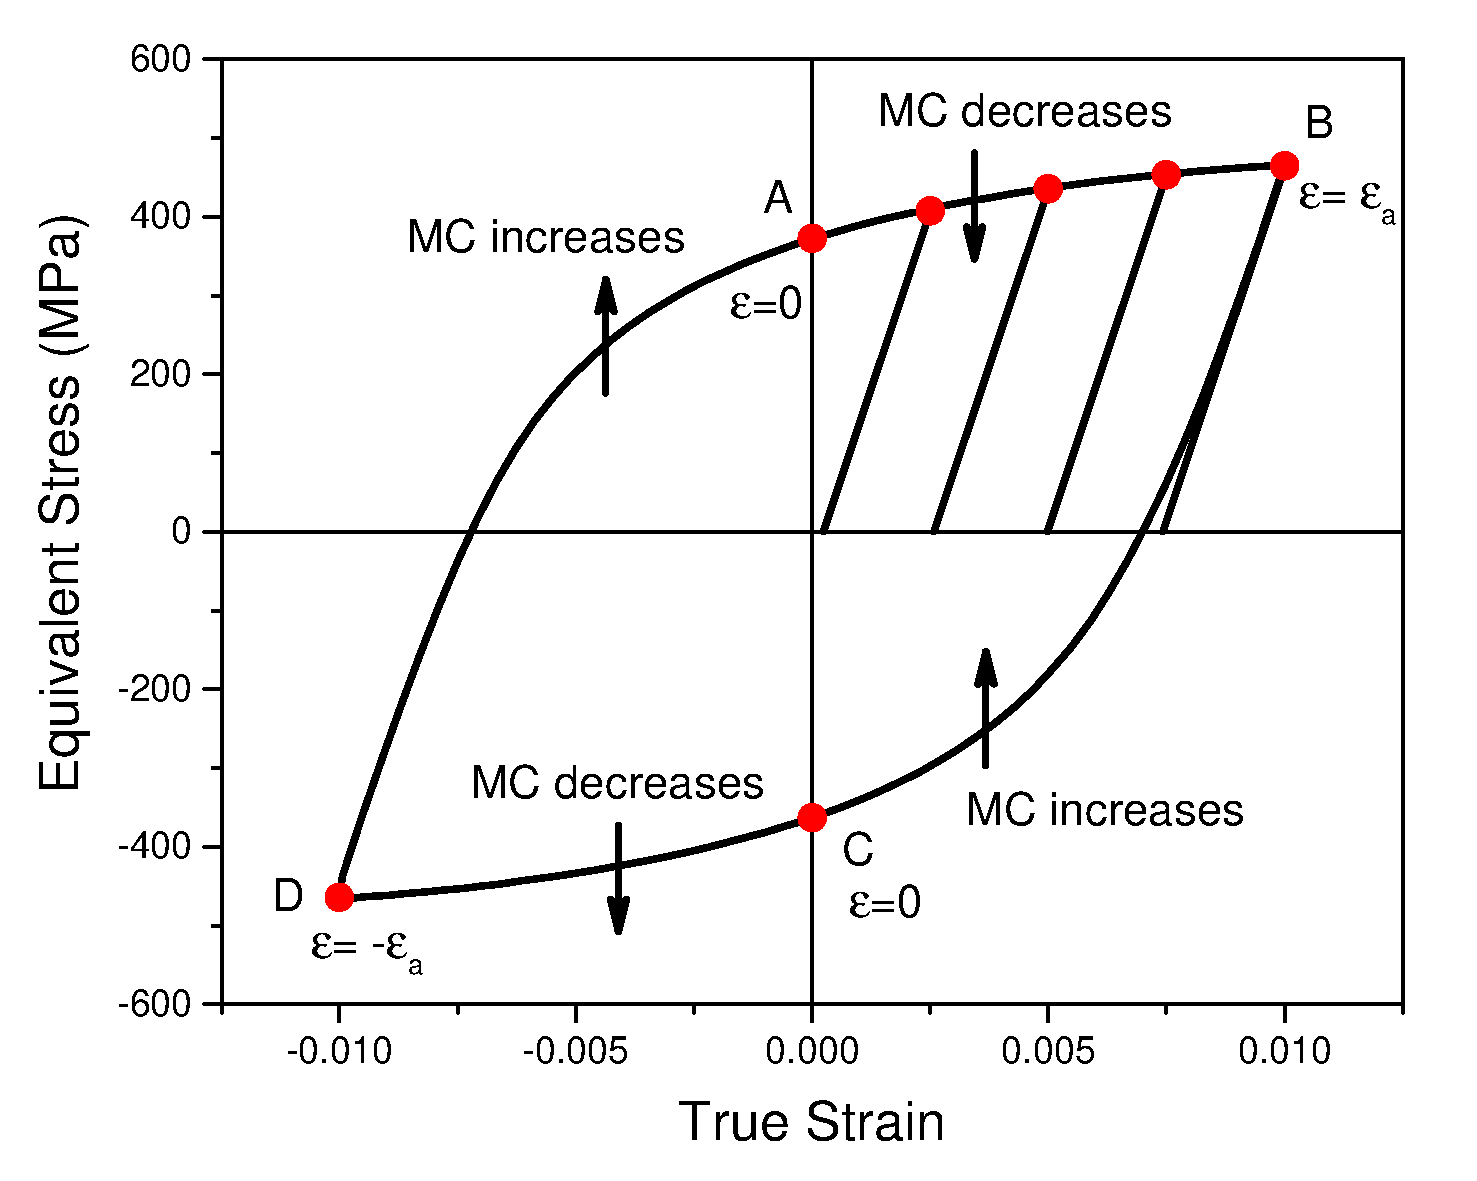
\includegraphics[width=8cm]{Steploadingcurve.pdf}
  \caption{Definition of measuring points in a loading cycle. A, B, C and D represent loading change points from loading to unloading.  Within a loading segment, e.g. A-B, several additional breaking points can be inserted to illustrate MC variations.}
  \label{fig:PointDefinition}
  \end{center}
\end{figure}

\begin{figure}[!h]
  \begin{center}
  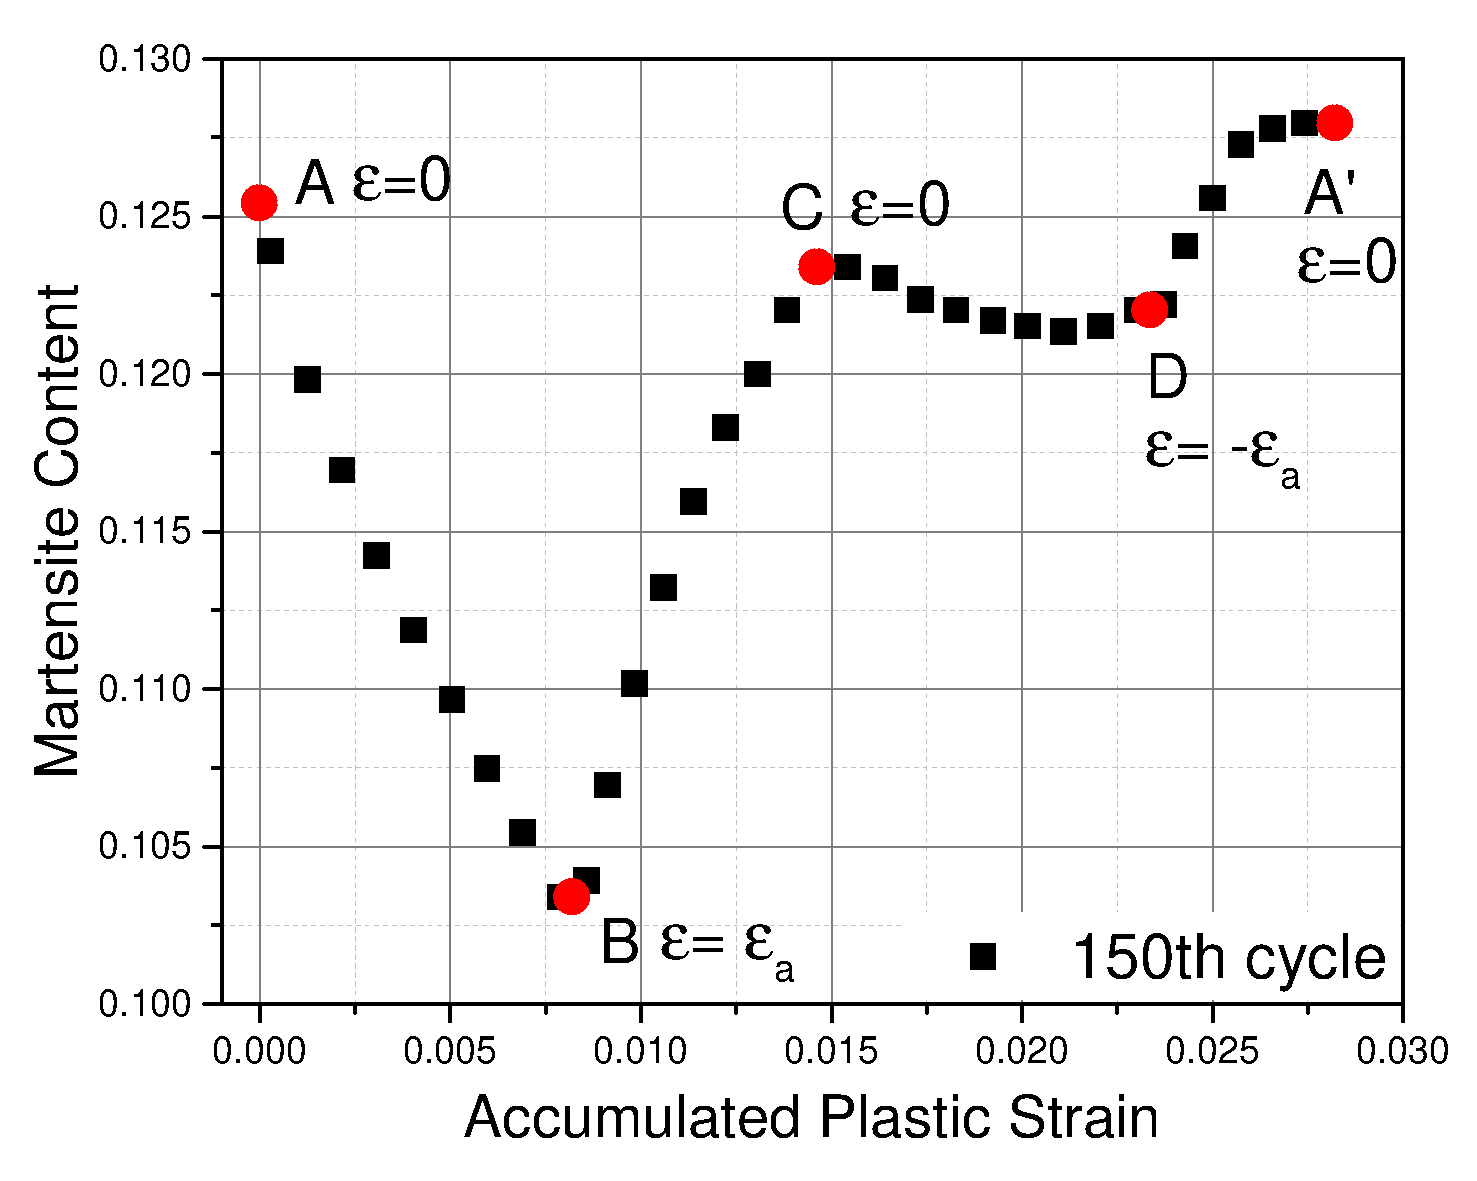
\includegraphics[width=8cm]{MCvariation.pdf}
  \caption{Variations of MC within the 150th cycle of a torsional cyclic loading test}
  \label{fig:Variations of martensite content}
  \end{center}
\end{figure}

%\begin{figure}[!h]
%  \begin{center}
%  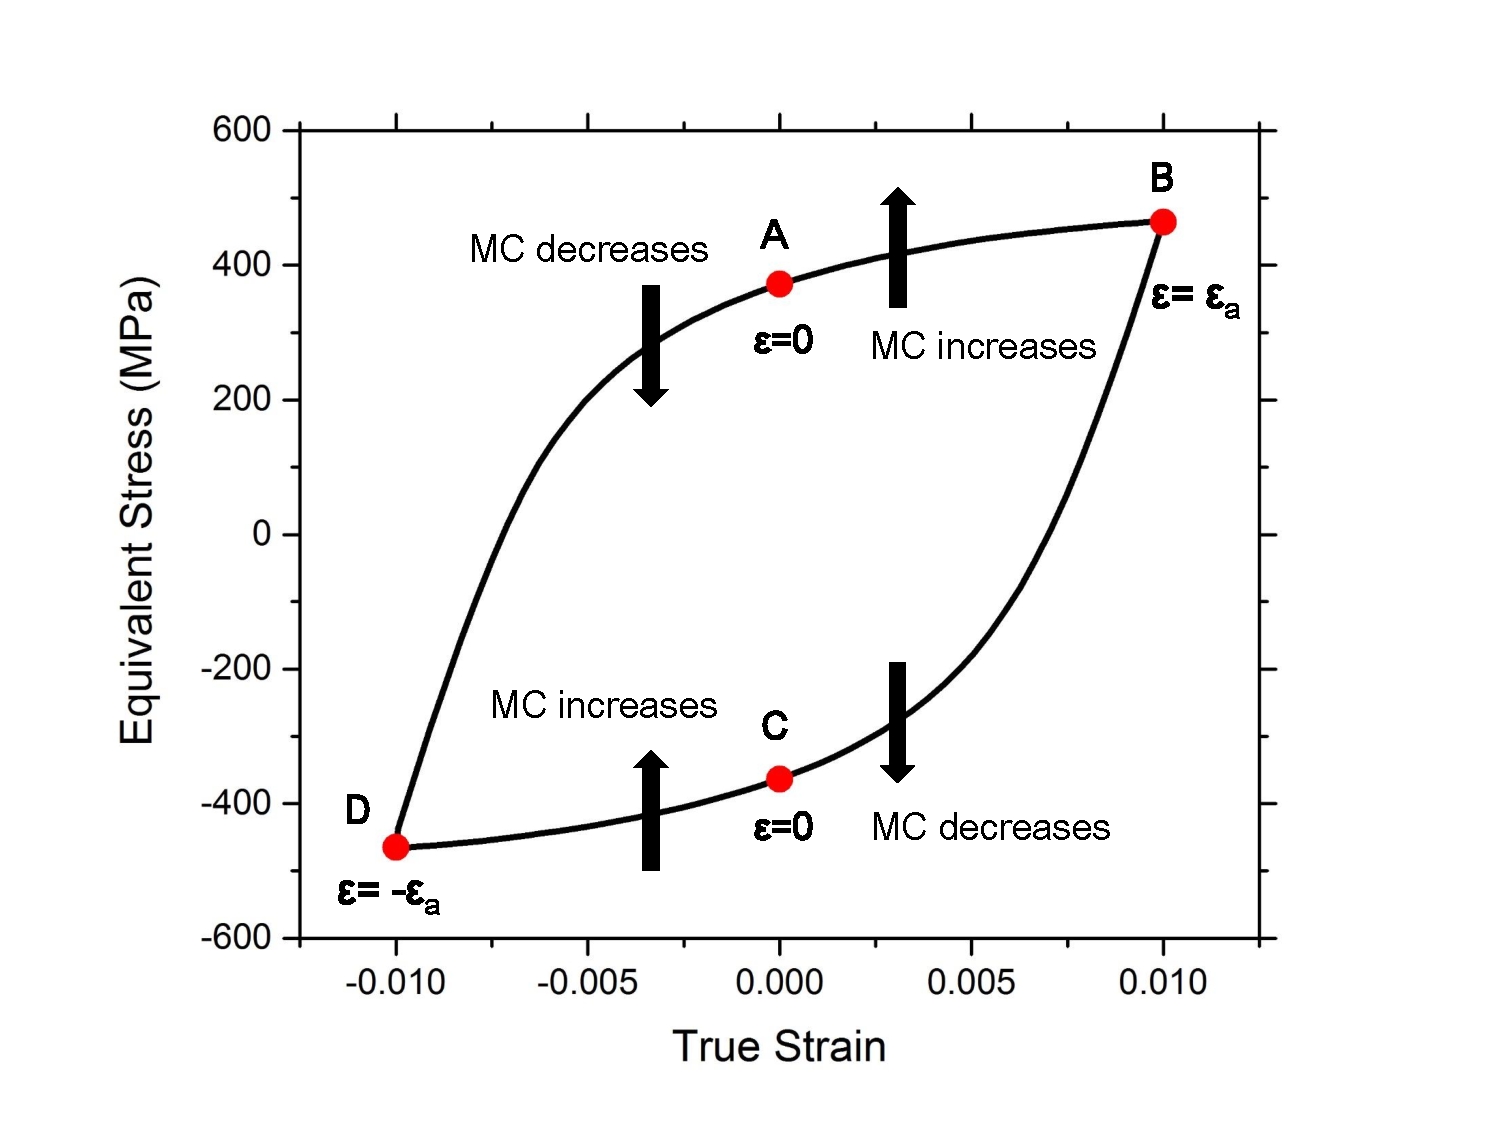
\includegraphics[width=8cm]{Steploadingfourpoints.pdf}
%  \caption{Cyclic secondary hardening value relation to the martensite content}
%  \label{fig:Steploadingfourpoints}
%  \end{center}
%\end{figure}

Variations of  MC within a cycle of a torsional cyclic loading test with $\varepsilon_{\rm a}=1.0\%$ was illustrated in Fig. \ref{fig:Variations of martensite content} (\marked{How was the situation under tension/compression, you should add at least one curve more into the figure, otherwise the figure is not conclusive.}).
The MC evolution within each loading cycles were studied through a series of loading/unloading steps, with $\varepsilon_{\rm a}=0.8\%,1.0\%,1.2\%$. It was observed that  MC would fluctuate during each cycles although the overall trend was that the martensite content increases after a complete cycle, as shown in the Fig. \ref{fig:PointDefinition}.
\marked{Within a loading cycle the evolution of MC follows such a process: (1) MC decreases with the increasing stress and plastic strain. (2) MC increases after stress release. The martensite forms under compressive plasticification. (3) MC decreases under compressive plastic deformations \marked{(This is also contradictory to the kinetics model)}.  (4) MC increases to the initial value and obtains a small amount of increment. It is interesting to see that the martensite content decreases when $\sigma \cdot \varepsilon_{\rm p} > 0$(???$\sigma \cdot \varepsilon > 0$)  and increases when  $\sigma \cdot \varepsilon_{\rm p}<0$. The increase of the martensite content could be attributed to the increase of accumulated plastic strain which was related to plastic deformation. However, the decrease of the martensite content revealed the reversion of strain-induced martensite and this phenomenon has been rarely reported. }




\begin{figure}[!h]
\centering
\subfigure[Step loading cyclic test with $\varepsilon_{\rm a}=0.8\%$]{
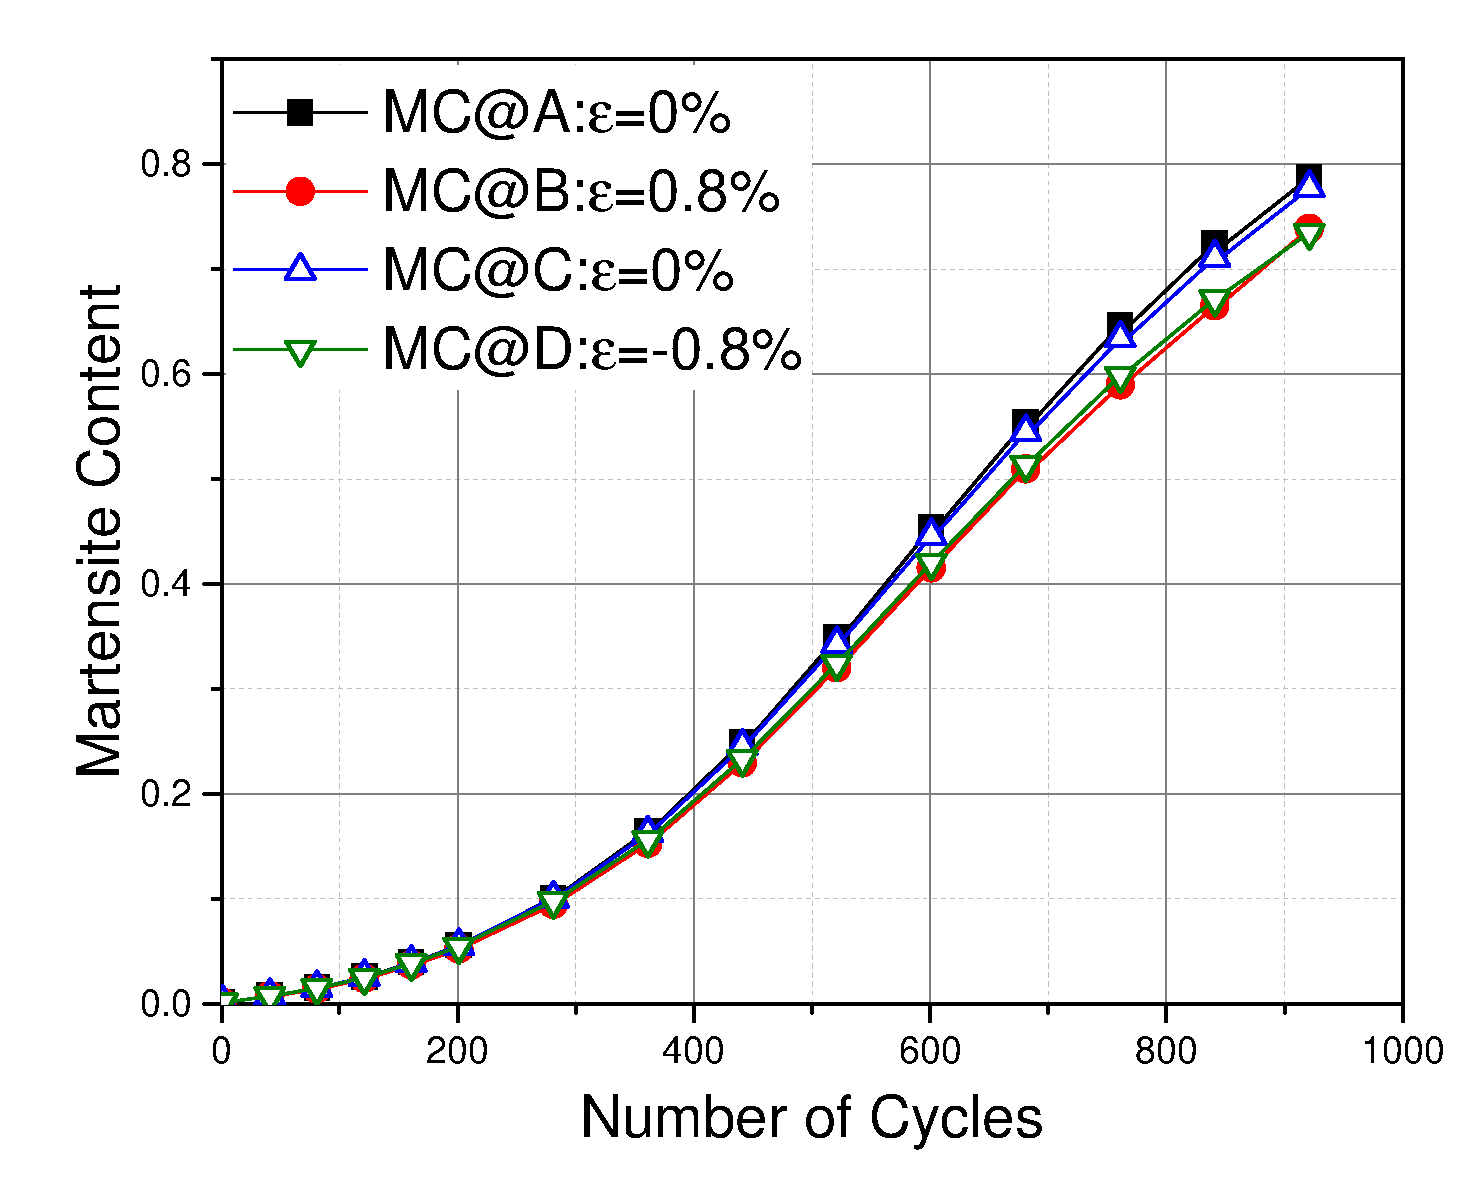
\includegraphics[width=8cm]{SteploadingTorsional08.pdf}
}
\quad
\subfigure[Step loading cyclic test with $\varepsilon_{\rm a}=1.0\%$]{
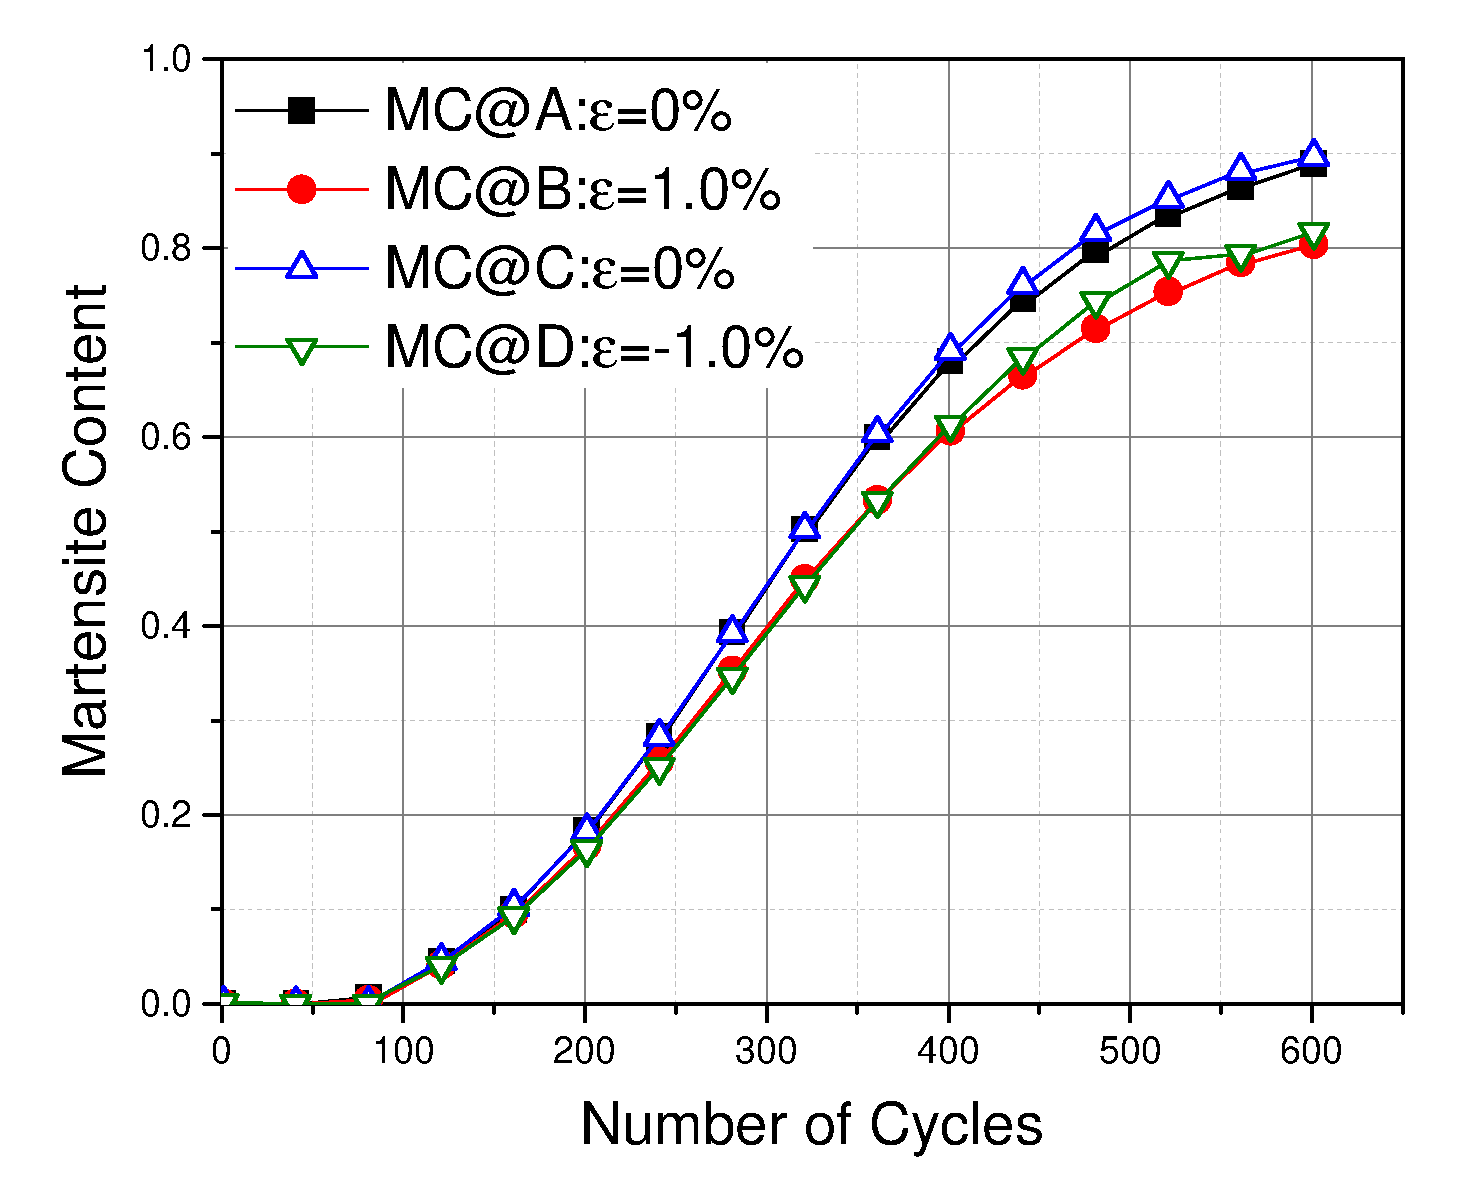
\includegraphics[width=8cm]{SteploadingTorsional10.pdf}
}
\quad
\subfigure[Step loading cyclic test with $\varepsilon_{\rm a}=1.2\%$]{
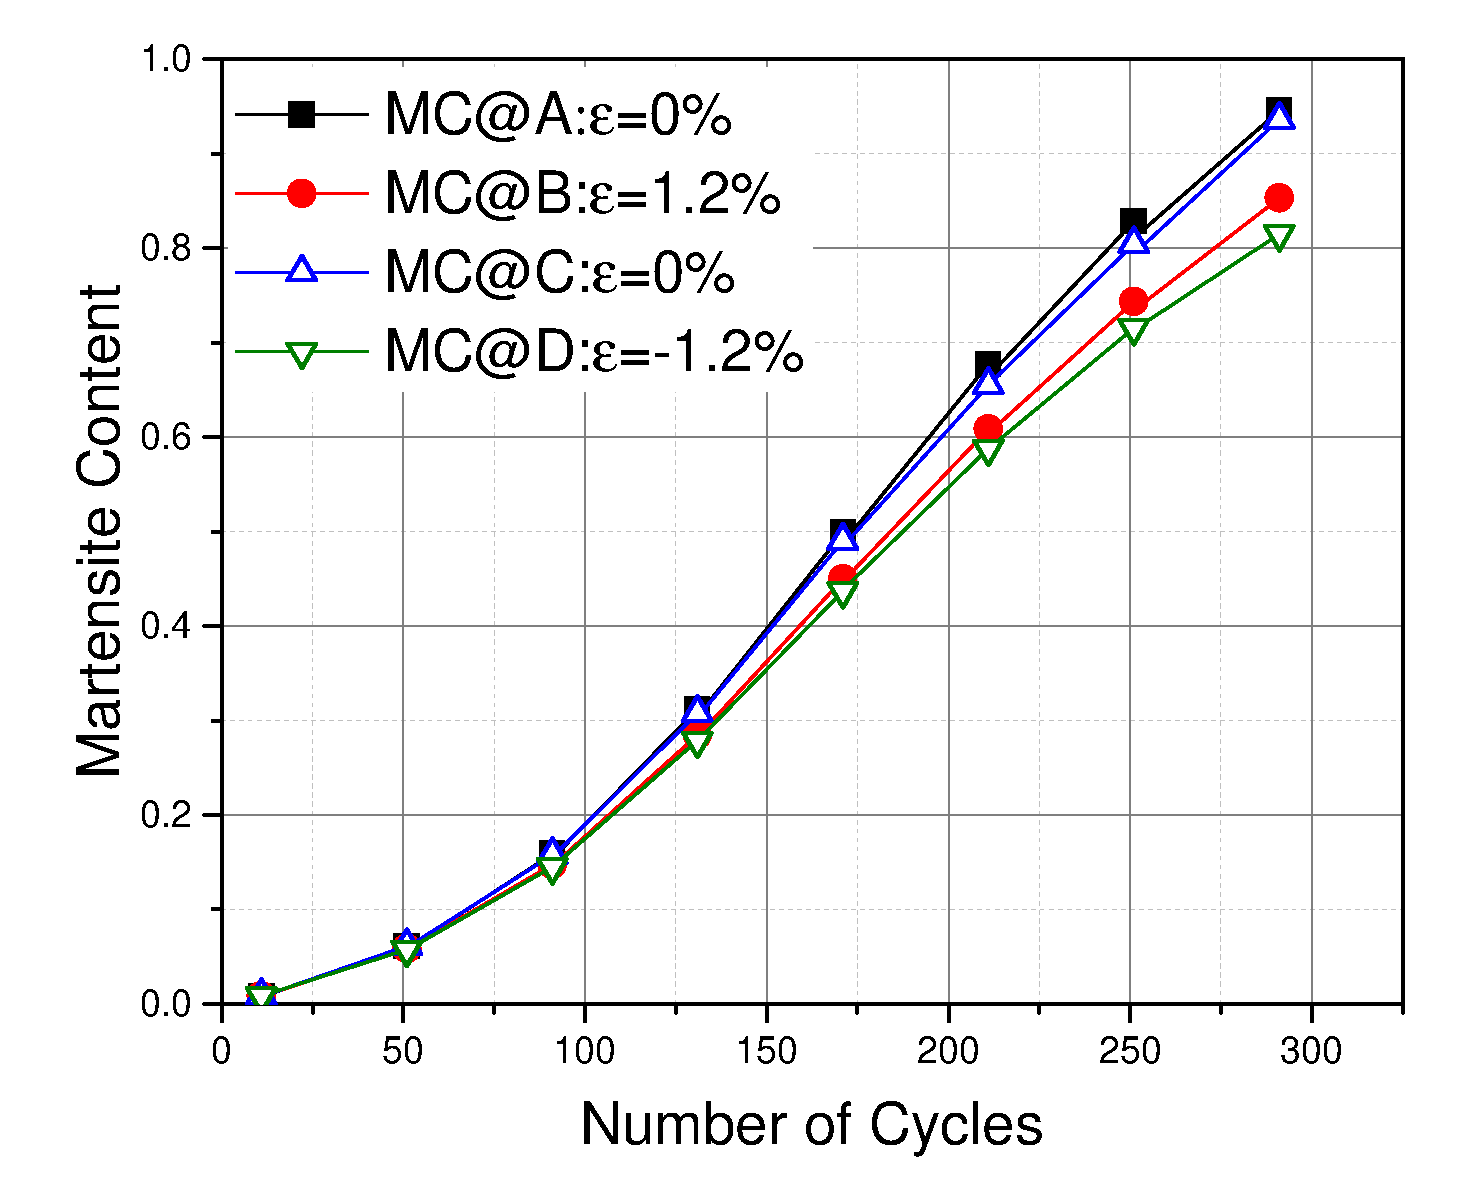
\includegraphics[width=8cm]{SteploadingTorsional12.pdf}
}
\caption{The fluctuations of the martensite contents in torsional cyclic loading processes. }
\label{fig:SteploadingTorsional}
\end{figure}

More experimental results for different loading amplitudes are summarized in Fig. \ref{fig:SteploadingTorsional}, for the whole cyclic loading history till failure. For each given loading amplitude, MC values at points A - D in Fig. \ref{fig:PointDefinition} are plotted. The martensite evolution displayed in the Fig. \ref{fig:total1} is the martensite content at point A of each loading cycles. \marked{It can be speculated that the actual martensite evolution during the cyclic loading tests is a sigmoidal curve with zigzags within each cycles. In addition, the relative amplitudes of the fluctuation of the martensite contents were quite stable respectively. For instance, the martensite content fluctuated within $3\%,5\%,6\%$ for step loading cyclic tests with $\varepsilon_{\rm a}=0.8\%,1.0\%,1.2\%$. Since the main purpose of the present paper is to establish a kinetics model for martensitic transformation under proportional cyclic loadings and construct a corresponding cyclic plasticity model, the fluctuation of the martensite content was relatively small enough to be neglected for previously mentioned cyclic loading tests. This fluctuation could be investigated in the further studies and a more accurate evolution kinetics can be then established.}
%(这段文字需要很好琢磨,尤其是和总体变化相反的现象需要有很好的解释。首先需要明确试验结果的正确性和可重复性,其次需要明确通过间接测量可能出现的问题和误差,再次需要研究载荷幅值和应力三轴度的影响,得出规律。这里只讨论试验,但试验结果必须相互协调。这个现象不是本文的重点,但既然提出来了,就不能出错、令人信服、得有结论。如果这个试验结果可信,那的确值得再次仔细研究研究,单独成文!)


\subsection{Effects of loading paths}
As shown in Fig. \ref{fig:total2}, evolution of martensitic transformation under the constant equivalent strain amplitude is independent of the tension or shear loads. An additional test with constant tension-torsional loading ratio $\varepsilon : \gamma /\sqrt{3}=1:1$ was performed and plotted together with uniaxial loading results in Fig.  \ref{fig:proportional1}. The proportional loading case is termed as LoadingPath3 in the figure, in which the horizontal axis is the equivalent strain. All three tests were run under the same equivalent strain range.

\begin{figure}[!h]
  \begin{center}
  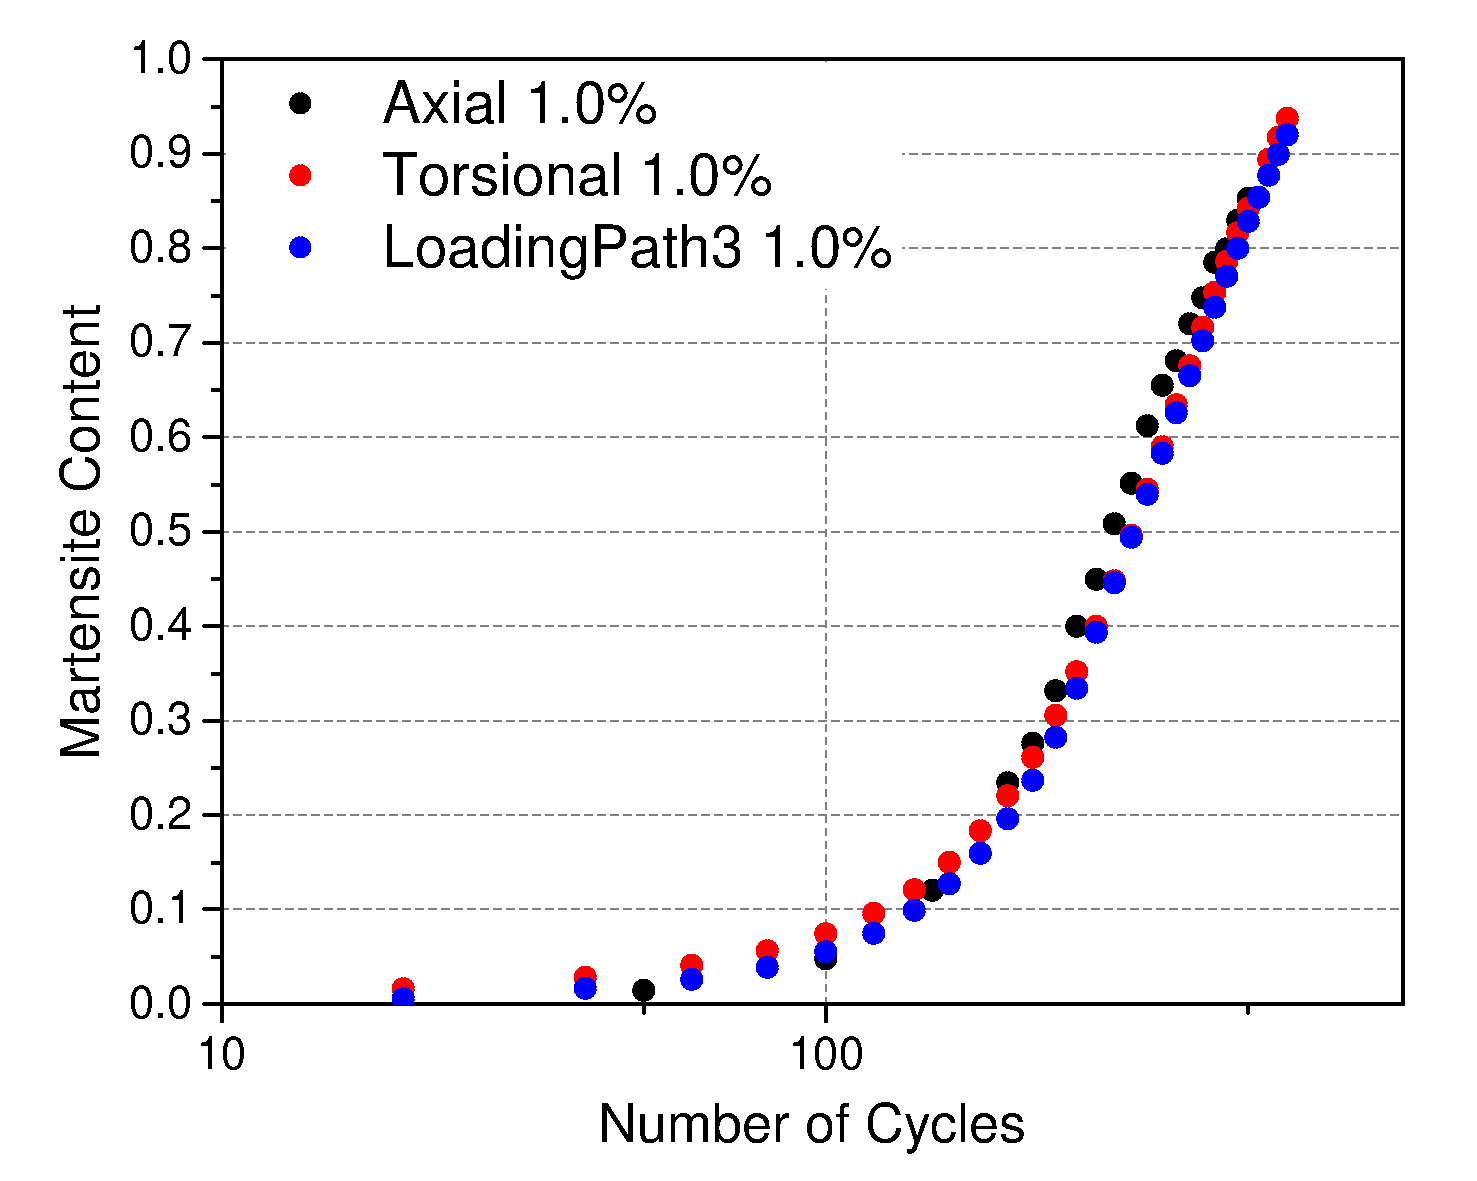
\includegraphics[width=8cm]{proportional1.pdf}
  \caption{Effects of loading configuration to development of the martensite content as a function of the loading cycle number. The unique correlation between the MC and cycle number implies independence between MC evolution and stress triaxiality, at least under proportional loading conditions.}
  \label{fig:proportional1}
  \end{center}
\end{figure}

The curves in Fig. \ref{fig:proportional1} imply that the evolution of the martensite content is not affected by biaxial loading configuration, i.e. the stress triaxiaity, at least for the proportional loading case. This prediction seems not to agree with observations under monotonic loading conditions (\citeauthor{Santacreu2006Behaviour}, \citeyear{Santacreu2006Behaviour}; \citeauthor{Beese2011Effect}, \citeyear{Beese2011Effect}; \citeauthor{Stringfellow1992A}, \citeyear{Stringfellow1992A}). For instance, it was reported in the metastable austenitic steels under monotonic loadings that the highest martensite developed under plane-strain tension, followed by simple tension, shear and simple compression, with the lowest martensite content developed under plane-strain compression (\citeauthor{Stringfellow1992A}, \citeyear{Stringfellow1992A}). \marked{In fact, the loading-path independent MC curves do show the sensitive stress variation and so also different plastic strain increments. That is, the MC as a function of the total strain amplitude can be considered as a function of the plastic strain amplitude and the elastic strain amplitude, the latter can be expressed by the stress. In this sense, the cyclic martensitic phase transformation does affected by both plastic strain and stress.}
same old talkings, does not make sense.

Experiments on a non-proportional loading path reveal that the MC development is a function of the stress, as shown in
Fig. \ref{fig:non-proportional and path}.
It is shown that the growth rate of the martensitic transformation under non-proportional loading path was much faster than that of proportional loading paths. This is reasonable because shear strain plays a more important role in the strain-induced martensitic transformation. Thus non-proportional loading path could result in the rotation of maximum shear plane which might lead to a faster growth of martensite in phase transformation.

\begin{figure}[!h]
  \begin{center}
  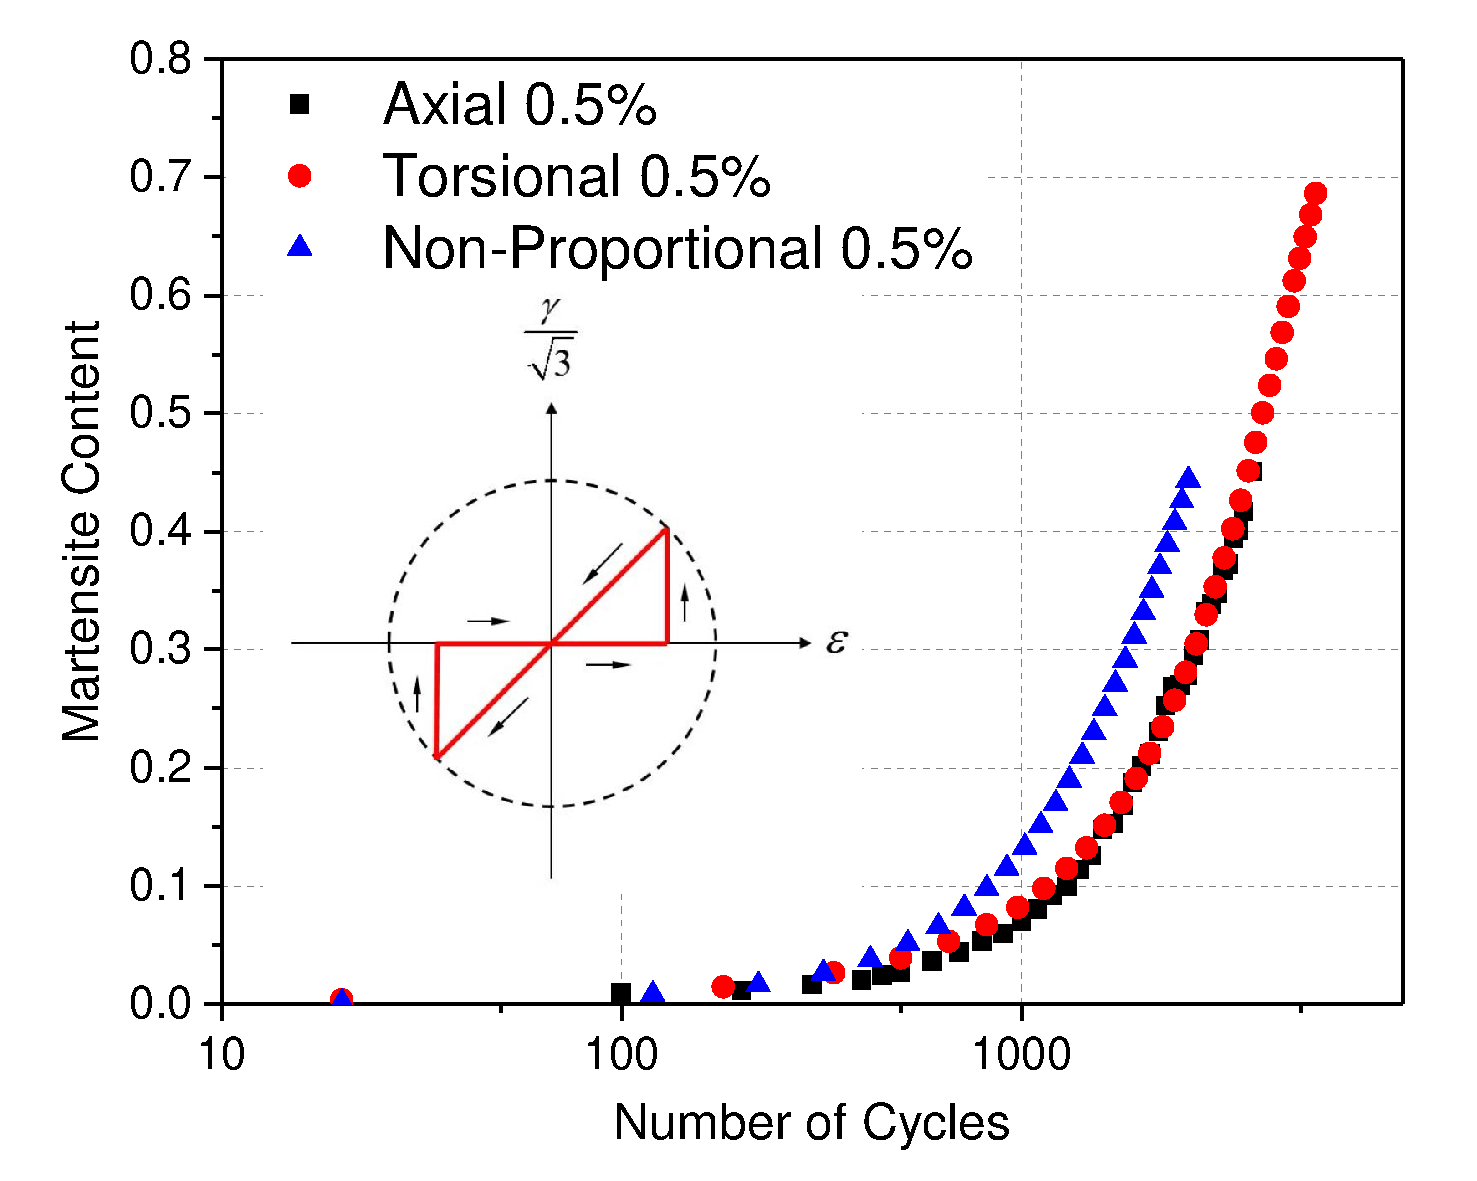
\includegraphics[width=8cm]{non-proportional2andpath.pdf}
  \caption{Effects of the non-proportional load to development of martensite phase with an equivalent strain amplitude of 0.5\%.}
  \label{fig:non-proportional and path}
  \end{center}
\end{figure}

In summary, it was natural to assume that the stress triaxiality needs to be considered in cyclic MC development. Both plastic strain and stress triaxiality change MC evolutions and are the driving forces to the phase transformation. The kinetics model for monotonic loadings  and cyclic loadings may share a similar mathematical form.


\section{Plasticity for austenitic steels with martensitic phase transformation}

\subsection{Kinetics for the martensitic phase transformation}
Most kinetics models for the martensitic transformation linked the martensite content with the equivalent plastic strain (under monotonic loadings) or accumulated plastic strain (under cyclic loadings). The accumulated plastic strain $p$ is defined as
\begin{equation}\label{eq:Accumulated plastic strain}
p=\int \sqrt{\frac{2}{3}{\dot\varepsilon _{ij}^{\rm p}\dot\varepsilon _{ij}^{\rm p}}}{\rm d}t.
\end{equation}
Above $\varepsilon _{ij}^{\rm p}$ denotes the plastic strain. $\dot x $ represents the time rate of the variable $x$. \cite{Santacreu2006Behaviour} described the phase transformation under monotonic loadings with equivalent strain and stress triaxiality, as
\begin{equation}\label{eq:Santacreu model}
\dot{\chi }= \left ( \chi _{\max} - \chi \right ) nD \left ( D \bar {\varepsilon}^{\rm p} \right )^{n-1}\dot{ \bar {\varepsilon }^{\rm p}},
\end{equation}
where $\chi$ is the martensite content and $\bar {\varepsilon }^{\rm p}$ is the equivalent plastic strain . $D$ and $n$ are model parameters which should be independent of temperature. The influence of stress triaxiality is implemented in $D$.

\cite{Beese2011Effect} conducted monotonic loading tests under different stress triaxialities and expanded on the basis of Santacreu model by adding the Lode angle  into the kinetics model,
\begin{equation}\label{eq:Beese model}
D\left ( \eta,\theta  \right )=\left ( D_{0}+a_{\eta}\eta+a_{\theta}\theta \right ),
\end{equation}
where $\theta$ is the Lode angle  and $\eta$ is the stress triaxiality. By linearly associating $D$ with the stress triaxiality and the Lode angle, this model could describe the martensitic transformation under monotonic loadings with different stress state including equi-biaxial tension, plain strain tension/compression, uniaxial tension/compression and pure shear cases.

For martensitic transformation under cyclic loadings, \cite{Smaga2008Deformation} established a fitting model by relating the MC with material parameters and strain amplitudes,
\begin{equation}\label{eq:Smaga model}
\chi =\chi _{\max}\left ( 1-e^{-\alpha p ^{n}} \right ),
\end{equation}
where $\alpha$ is a parameter related with strain amplitude and material, $n$ is additional fitting parameter to meet experimental data. \cite{Smaga2008Deformation} used a simplified equation $p= N { \varepsilon _{\rm a,p}}$ to calculate the accumulated plastic strain within $N$ loading cycles, in which $\varepsilon _{\rm a,p}$ is the amplitude of plastic strain calculated from applied strain amplitude, without considering cyclic hardening/softening in the material. Since the stress amplitude changes significantly with loading cycles, as shown in Fig. \ref{fig:total1}, the amplitude of the plastic strain varies dramatically for constant total strain amplitudes in the tests. In the present work the plastic strain $p=\sum \varepsilon _{\rm a,p}=\sum (\varepsilon_{\rm a} - \sigma_{\rm a}/E)$ with $\sigma_{\rm a}$ as the stress amplitude measured in experiments.
Evolutions of the martensite content versus accumulated equivalent plastic strain of the cyclic loading tests are shown in Fig. \ref{fig:EvolutionModel3}.

\begin{figure}[ht]
  \begin{center}
  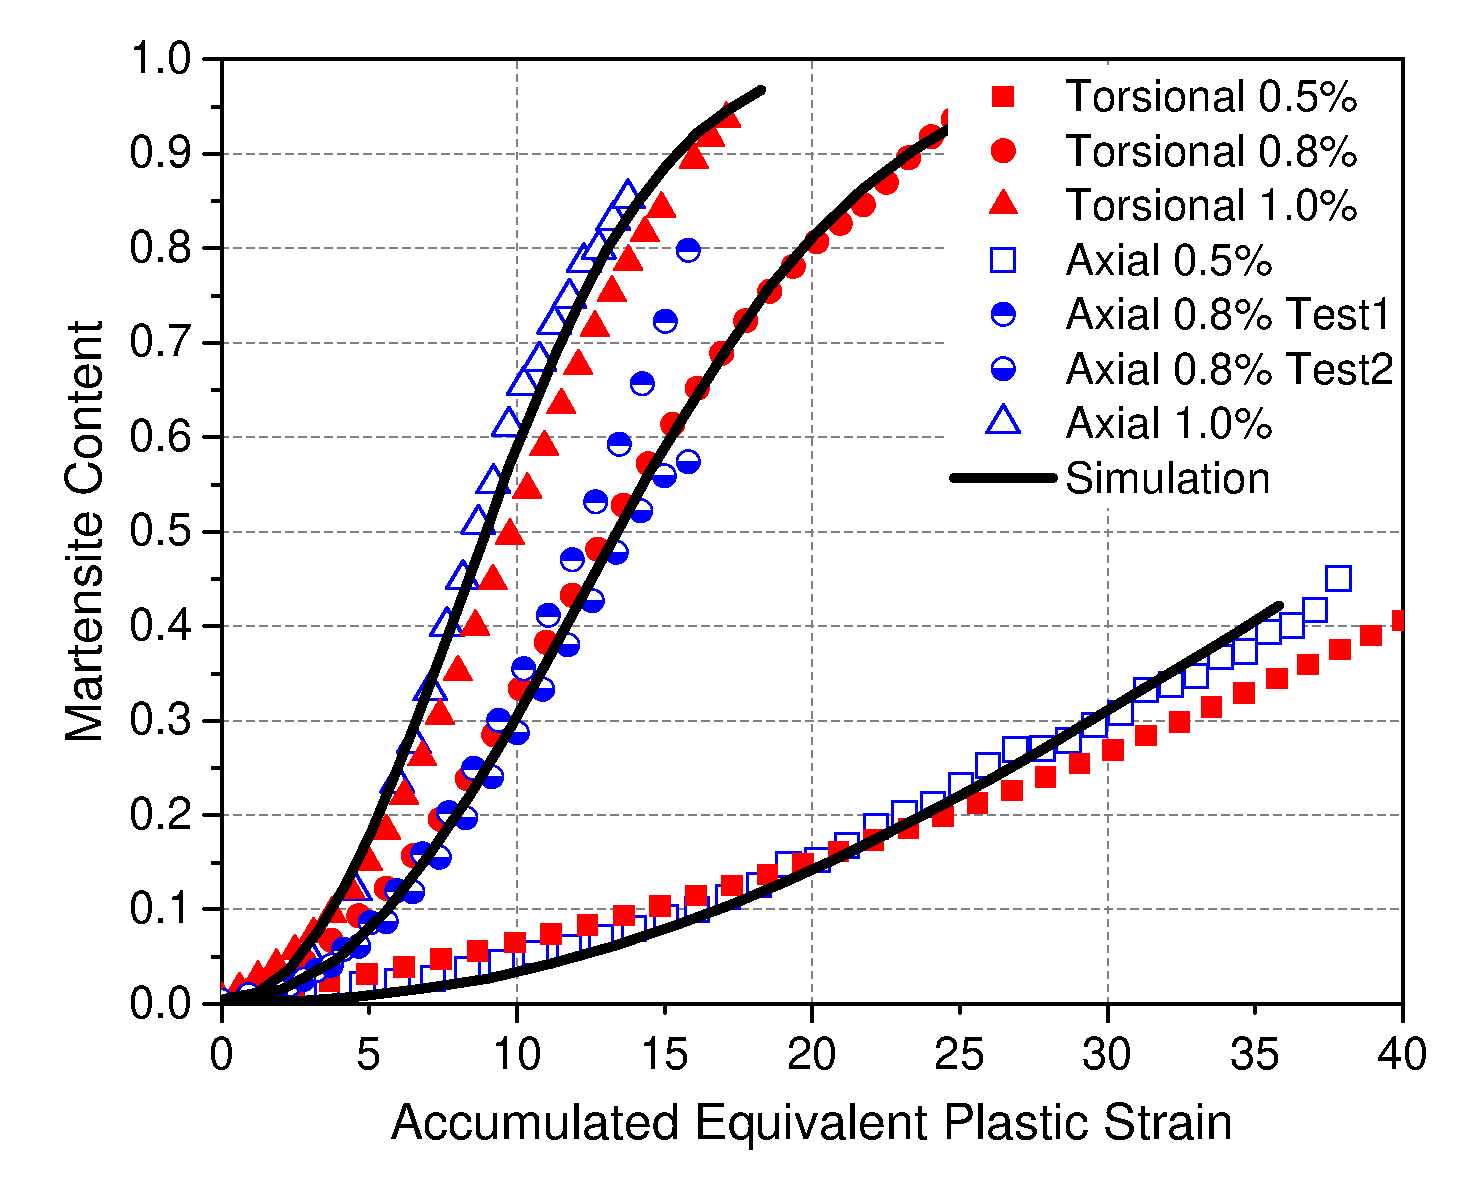
\includegraphics[width=8cm]{EvolutionModel3.pdf}
  \caption{The evolution of martensite content versus accumulated equivalent plastic strain in the present work and the comparison with martensite content obtained by kinetics model.}
  \label{fig:EvolutionModel3}
  \end{center}
\end{figure}

%\marked{(以下文字我基本没改,但公式、图我都调整了。主要是没想明白,无从下手,许多句子看不懂什么意思,比如这一段的第一句。这几点大家改一下:1. 试验已经证明了单调和循环相变驱动力的差异,还能视而不见吗?2. 这里模型相对很简单,真能重现全部试验结果?算一算比例加载过程。3. 塑性模型如何写你们讨论一下,现在这样太拖,打回的可能很大。)}

 It is evident that the evolutions of MC under the same equivalent strain amplitudes are consistent respectively(Fig. \ref{fig:EvolutionModel3}). However, the effect of strain amplitudes should not be simplified as a fitting parameter in the kinetics model. Such kinetics models are insufficient for establishing a constitutive model for the material. Instead, a variable which can solely describe the martensitic transformation needs to be found. It was reported that a certain value of plastic strain must be exceeded to trigger the martensitic transformation in AISI304L stainless steel (\citeauthor{Bayerlein1989Plasticity}, \citeyear{Bayerlein1989Plasticity}). This threshold was found to be $\Delta \varepsilon _{\rm p}/2=0.3\%$. Therefore, it was assumed that there were thresholds of plastic strain for martensitic transformation in AISI 348 under cyclic loadings and a kinetics model was developed. Deriving from the Santacreu-type model of martensitic transformation under monotonic loadings (\citeauthor{QSP2014}, \citeyear{QSP2014}), the present newly developed kinetics model can describe martensitic transformation under various loading conditions. The expression of the model is displayed below:
\begin{eqnarray}\label{eq:Kinetics model3}
\dot \chi &=&\left(\chi_{\max }-\chi\right) nD \left(D p_{\rm eff}\right)^{n-1}\dot p_{\rm eff},
\\
\dot{p}_{\rm eff}&=&k\left ( \bar{\varepsilon}_{\rm p} \right ) \cdot H\left(\bar{\varepsilon}_{\rm p}-\varepsilon_{\rm p}^{\rm th}\right) \dot{p} ,
\\
k\left ( \bar{\varepsilon}_{\rm p} \right )&=&1-\exp \left[-a\left(\bar{\varepsilon}_{\rm p}^{\rm peak}-\varepsilon_{\rm p}^{\rm th}\right)^{m}\right] ,
\\
D&=&D_{0}+D_{1}\eta,
\end{eqnarray}
where $\varepsilon_{\rm p}^{\rm th}$ is the threshold value of the equivalent plastic strain to activate the martensitic transformation, $\varepsilon_{\rm p}^{\rm peak}$ is the peak value of the equivalent plastic strain in the lateset cycle, $\chi_{\max}$ is the maximum value of martensite content grown after the transformation in the material (or saturation value of martensite content), parameters $a,m,n$ are material constants and $H\left  ( x \right )$ (Heaviside step function) is equal to 1 when $x\geq0$. Parameter $D$ is a variable which describes the influence of the stress state by stress triaxiality $\eta$ through a linear correlation. The effective accumulated plastic strain $\dot{p}_{\rm eff}$ is defined as the accumulated plastic strain which directly decides the growth rate of the martensitic transformation. Since the plastic deformation is relatively more severe under monotonic loadings comparing with that of cyclic loadings with same amount of martensite transformed, the growth rate of martensite content versus the rate of accumulated plastic strain is much larger in monotonic conditions. Parameter $k$ is such a variable which distinguishes the influence to the growth rate of the cyclic loading paths from monotonic loadings.

The present kinetics model can degenerate into
\begin{equation}
\chi=\chi_{\max }\left(1-e^{-(D \overline{\varepsilon})^{n}}\right),
\end{equation}to describe the martensitic transformation under monotonic loadings. In details, $\varepsilon_{\rm p}^{\rm peak}$ can be considered as infinite under monotonic loading, thus $k$ equals to 1. Additionally, $\dot{p}_{\rm eff}=\dot{p}$ since the value of $\varepsilon_{\rm p}^{\rm th}$ is too small comparing with the plastic strain. As a result, the present kinetics model is applicable under both cyclic loadings and monotonic loadings. The values of model parameters are displayed in Table \ref{tab:Kinetics Model Parameters}.


\begin{table}[ht]
\centering
\caption{Kinetics model parameters (strain unit: mm/mm)}
\begin{tabular}{lllllll}
\hline
$\chi_{\max}$  &$n$       &$\varepsilon_{\rm p}^{\rm th}$ & $a$        & $m$        & $D_{0}$ & $D_{1}$ \\ \hline
1.0                 &2.22  &0.0012                            & 1.317 & 0.636  & 2.62        & 0.57  \\ \hline
\end{tabular}
\label{tab:Kinetics Model Parameters}
\end{table}


The evolutions of martensite content predicted by the model under cyclic loadings are in excellent accordance with the experimental results  (Fig. \ref{fig:EvolutionModel3}). If the material is subjected to monotonic loadings, the kinetics model degenerates into a more simplified Santacreu-style model (\citeauthor{QSP2014}, \citeyear{QSP2014}) which can well describe the martensitic transformation under monotonic loadings. Corresponding results are displayed in Fig. \ref{fig:EvolutionModel3formonotonic}.


\begin{figure}[ht]
  \begin{center}
  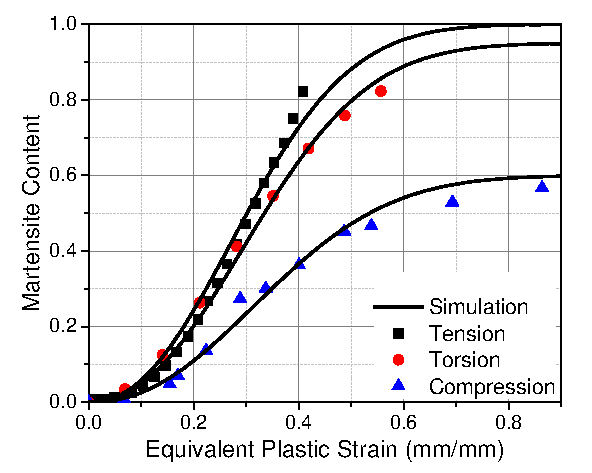
\includegraphics[width=8cm]{QinResult.pdf}
  \caption{Comparison of martensite content obtained by kinetics model and monotonic loading test results provided in reference(\citeauthor{QSP2014}, \citeyear{QSP2014})}
  \label{fig:EvolutionModel3formonotonic}
  \end{center}
\end{figure}

\subsection{Cyclic plasticity accounting for martensitic phase transformation}

Cyclic plasticity model can be simply divided into isotropic hardening and kinematic hardening. The isotropic hardening is commonly described by the change of yield stress while the back stress is used for kinematic hardening. In the case of monotonic loading, it is often reasonable to assume that only isotropic hardening occurred. However, this is often not appropriate for the case of cyclic loadings because of the Bauschinger effect. In kinematic hardening, the yield surface translates in stress space rather than expanding (like isotropic hardening). As a result, the yield function describing the yield surface is correlated to the location of the surface in stress space, Eq.  (\ref{eq:Yield Function}).
\begin{equation}\label{eq:Yield Function}
F=\sqrt{\frac{3}{2}\left ( \mathbf{s}-\mathbf{a} \right ):\left ( \mathbf{s}-\mathbf{a} \right )}-Y=0
\end{equation}
The back stress $\mathbf{a}$ is defined in the kinematic hardening and its evolution must be included in the model. The simplest linear kinematic hardening model was proposed by Prager (\citeauthor{Prager}, \citeyear{Prager}) and the evolution of back stress is collinear with the evolution of plastic strain, Eq. (\ref{eq:Prager model}).
\begin{equation}\label{eq:Prager model}
\dot{\mathbf{a}}=\frac{2}{3}c\dot{\bfepsilon}^{\rm p}
\end{equation}
where $c$ is a material constant. \cite{Frederick2007A} introduced a better description by introducing a recall term called dynamic recovery, Eq. (\ref{eq:AF model}).
\begin{equation}\label{eq:AF model}
\dot{\mathbf{a}}=\frac{2}{3} c \dot{\bfepsilon}^{\rm p}-\gamma \mathbf{a} \dot{p}
\end{equation}
where $c, \gamma$ are material constants. The second term on the right is called the recall term which is collinear with back stress $\mathbf{a}$ and is proportional to the norm of the plastic strain rate. The evolution of back stress $\mathbf{a}$ is then exponential for a monotonic uniaxial loading with a saturation value equals $c/ \gamma$.

Another approximation as shown in Eq. (\ref{eq:Chaboche model1983}) was postulated by \cite{Chaboche1983On} and the total back stress is composed of additive parts such as Eq. (\ref{eq:AF model}).
\begin{eqnarray}\label{eq:Chaboche model1983}
\dot{\mathbf{a}}^{k}&=&\frac{2}{3}c^{k}\dot{\{\bfepsilon}^{\rm p}-\gamma^{k} \mathbf{a}^{k}\dot{p}\\
\mathbf{a}&=&\sum_{k}^{M}\mathbf{a}^{k}
\end{eqnarray}
where $\mathbf{a}^{k}$ symbolizes the components of the total back stress $\mathbf{a}$ and $M$ is the number of the components considered. Another back stress model proposed by \cite{Chaboche1991On} introduced a threshold of back stress $\left\|\mathbf{a}^{k}\right\|$ to control the dynamic recovery term, Eq. (\ref{eq:Chaboche model1991}).
\begin{eqnarray}\label{eq:Chaboche model1991}
\dot{\mathbf{a}}^{k}&=&\frac{2}{3} c^{k} \dot{\bfepsilon}^{\mathrm{p}}-\gamma^{k}\left\langle 1-\frac{\mathbf{a}^{k}}{\left\|\mathbf{a}^{k}\right\|}\right\rangle \mathbf{a}^{k} \dot{p}\\
\left\|\mathbf{a}^{k}\right\|&=&\sqrt{\mathbf{a}^{k} : \mathbf{a}^{k}}
\end{eqnarray}
\cite{Ohno1993Kinematic} assumed that each component had a critical state for its dynamic recovery term to be activated fully and formulated kinematic hardening rules on the basis of Eq. \ref{eq:Chaboche model1991}. The total back stress is composed of additive parts:
\begin{equation}
\dot{\mathbf{a}}=\sum_{k=1}^{M} \dot{\mathbf{a}}^{k}
\end{equation}

The evolutions of back stress components $\dot{\mathbf{a}}^{k}$ take two forms as following.

$\textbf{Model I}$: the extreme case, corresponding to some multilinear model. It was assumed that the dynamic recovery term would not be fully activated until its magnitude attained a critical value which resulted from the energy required for cross slip. The critical state is introduced by a surface $f^{k}=\left\|\mathbf{a}^{k}\right\|-c^{k} / \gamma^{k}=0$. The dynamic recovery term operates only when the back stress attains this surface. Under proportional loadings, It writes:
\begin{equation}\label{eq:Ohno Wang model 1}
\dot{\mathbf{a}}^{k}=\frac{2}{3}c^{k}\dot{\bfepsilon}^{\rm p}-\gamma^{k} H\left ( f^{k} \right )\left \langle \dot{\bfepsilon}^{\rm p}: \frac{\mathbf{a}^{k}}{\left \| \mathbf{a}^{k} \right \|}\right \rangle\mathbf{a}^{k}\\
\end{equation}
where $H\left( \right)$ is the Heaviside step function and the Macaulay bracket introduces the consistency condition for the critical state $f^{k}=\dot{f}^{k}=0$.

$\textbf{Model II}$: the smooth version, more realistic, replaces the Heaviside step function by a power function. It was assumed that the dynamic recovery term would become significantly nonlinearly as $\left\|\mathbf{a}^{k}\right\|$ approaches the surface $f^{k}=0$. It writes:
\begin{equation}\label{eq:Ohno Wang model 2}
\dot{\mathbf{a}}^{k}=\frac{2}{3} c^{k} \dot{\bfepsilon}^{\mathrm{p}}-\gamma^{k}\left(\frac{\left\|\mathbf{a}^{k}\right\|}{c^{k} / \gamma^{k}}\right)^{m^{k}}\left \langle \dot{\bfepsilon}^{\rm p}: \frac{\mathbf{a}^{k}}{\left \| \mathbf{a}^{k} \right \|}\right \rangle
\end{equation}
Though not necessary, the Macaulay bracket $\left\langle\dot{\varepsilon}^{\rm p} : \frac{\mathbf{a}^{k}}{\left\|\mathbf{a}^{k}\right\|}\right\rangle$ continues to operate in this smooth version, and will play a significant role in reducing ratchetting.

In the present paper, it is suggested that the martensitic transformation would only influence the isotropic hardening part by yield stress $Y=Y_{0}+Y_{pt}$. In addition, it is assumed that the kinematic hardening and cyclic hardening parts are inherent characters of the material without phase transformation. Since the non-proportional loading path is not considered in this study, its effect to the isotropic hardening is excluded in the model. Observations on stress-strain hysteresis loops of the AISI 348 specimens showed that the peak stresses were not monotonic to plastic strain (Fig. \ref{fig:total1}). The alloy demonstrated initially cyclic softening behavior and then cyclic hardening. However, the effect of cyclic softening behavior to the stress amplitudes was less than $10\%$ with an average effect not over $5\%$. As a result, it is reasonable to neglect this cyclic softening behavior and focus on the cyclic hardening. In order to describe such complex behavior, $c^{k}$ could be divided into two parts (\citeauthor{Fang2015Cyclic}, $c_{0}^{k}$ and $c_{\Delta}^{k}$. Variable $c_{\Delta}^{k}$ is assumed to depend on the accumulated plastic strain. The dependence on plastic strain allows more accurate description of the cyclic hardening behavior of the material. The kinematic hardening part is based on the model II of Ohno-Wang model (\citeauthor{Ohno1993Kinematic}, \citeyear{Ohno1993Kinematic}) and 3 back stress components are selected.


The model parameters are determined by the monotonic and cyclic stress-strain curves. For example, the parameters $c_{0}^{k}$ can be decided by neglecting the plastic strain amplitude effect since the cyclic hardening and multiaxial effect are absent in the monotonic tensile test. It was recommended (\citeauthor{Jiang1996Characteristics}, \citeyear{Jiang1996Characteristics}; \citeauthor{Jiang1996Modeling}, \citeyear{Jiang1996Modeling}) that $c_{0}^{k}\left  ( k=1,2,3 \right )$ could be determined by Eq. (\ref{eq:Cyclic hardening parameter by monotonic curve})
\begin{equation}\label{eq:Cyclic hardening parameter by monotonic curve}
c_{0}^{k}=\left (\frac{\sigma^{k}-\sigma^{k-1}}{\varepsilon_{\mathrm{p}}^{k}-\varepsilon_{\mathrm{P}}^{k-1}}
-\frac{\sigma^{k+1}-\sigma^{k}}{\varepsilon_{\mathrm{P}}^{k+1}-\varepsilon_{\mathrm{p}}^{k}}\right)
\end{equation}
where $\sigma^{k}$ and $\varepsilon_{\rm p}^{k}$ denote the stress and plastic strain at the k-th point on the monotonic stress-plastic strain curve respectively. $\sigma^{0}$ is the initial yield stress related to the zero plastic strain $\varepsilon_{\rm p} = 0$. Generally, the uniaxial tensile stress-strain curve is represented in 4 sections in the present paper.

In the constitutive model, the saturated value of $c^{k}$ has to be determined from the cyclic stress-strain curve, which can be obtained from the experimental stabilized hysteresis loop. Since the stress-strain curve of AISI 348 changes ceaselessly, the half fatigue life $\left (N_{\mathrm{f}} / 2\right)$ cycle is assumed to be the stabilized hysteresis loop instead. The stress-strain curve in the stabilized hysteresis loop can be divided into a stress increasing section and a stress decreasing section. The alternating values of stress and strain were calculated by taking half of the absolute value between a data point and the starting point (\citeauthor{SunCyclic}, \citeyear{SunCyclic}). The alternating stress and strain relation of the stress increasing part and the stress decreasing part can be expressed in the function $f_{\rm  inc } (\sigma, \varepsilon)$ and $f_{\rm { dec }} (\sigma, \varepsilon)$ respectively. The final alternating stress-strain curve is obtained by combining these two functions, as demonstrated in Fig. \ref{fig:Alternating Curve} and Eq. (\ref{eq:AlternatingCurve}).
\begin{eqnarray}\label{eq:AlternatingCurve}
f_{\rm { inc }}^{\rm {alter}} (\sigma, \varepsilon)&=&f_{\rm { inc }} (\left|2 \sigma-\sigma_{\min }\right|, \left|2 \varepsilon-\varepsilon_{\min }\right|)\\
f_{\rm { dec }}^{\rm {alter}}(\sigma, \varepsilon)&=&f_{\rm { dec }}(\left|2 \sigma-\sigma_{\min }\right|, \left|2 \varepsilon-\varepsilon_{\min }\right|)\\
f(\sigma, \varepsilon)&=&\frac{1}{2}\left(f_{\rm { inc }}^{\rm {alter}}(\sigma, \varepsilon)+f_{\rm { dec }}^{\rm {alter}}(\sigma, \varepsilon)\right)
\end{eqnarray}
\begin{figure}[htbp]
  \begin{center}
  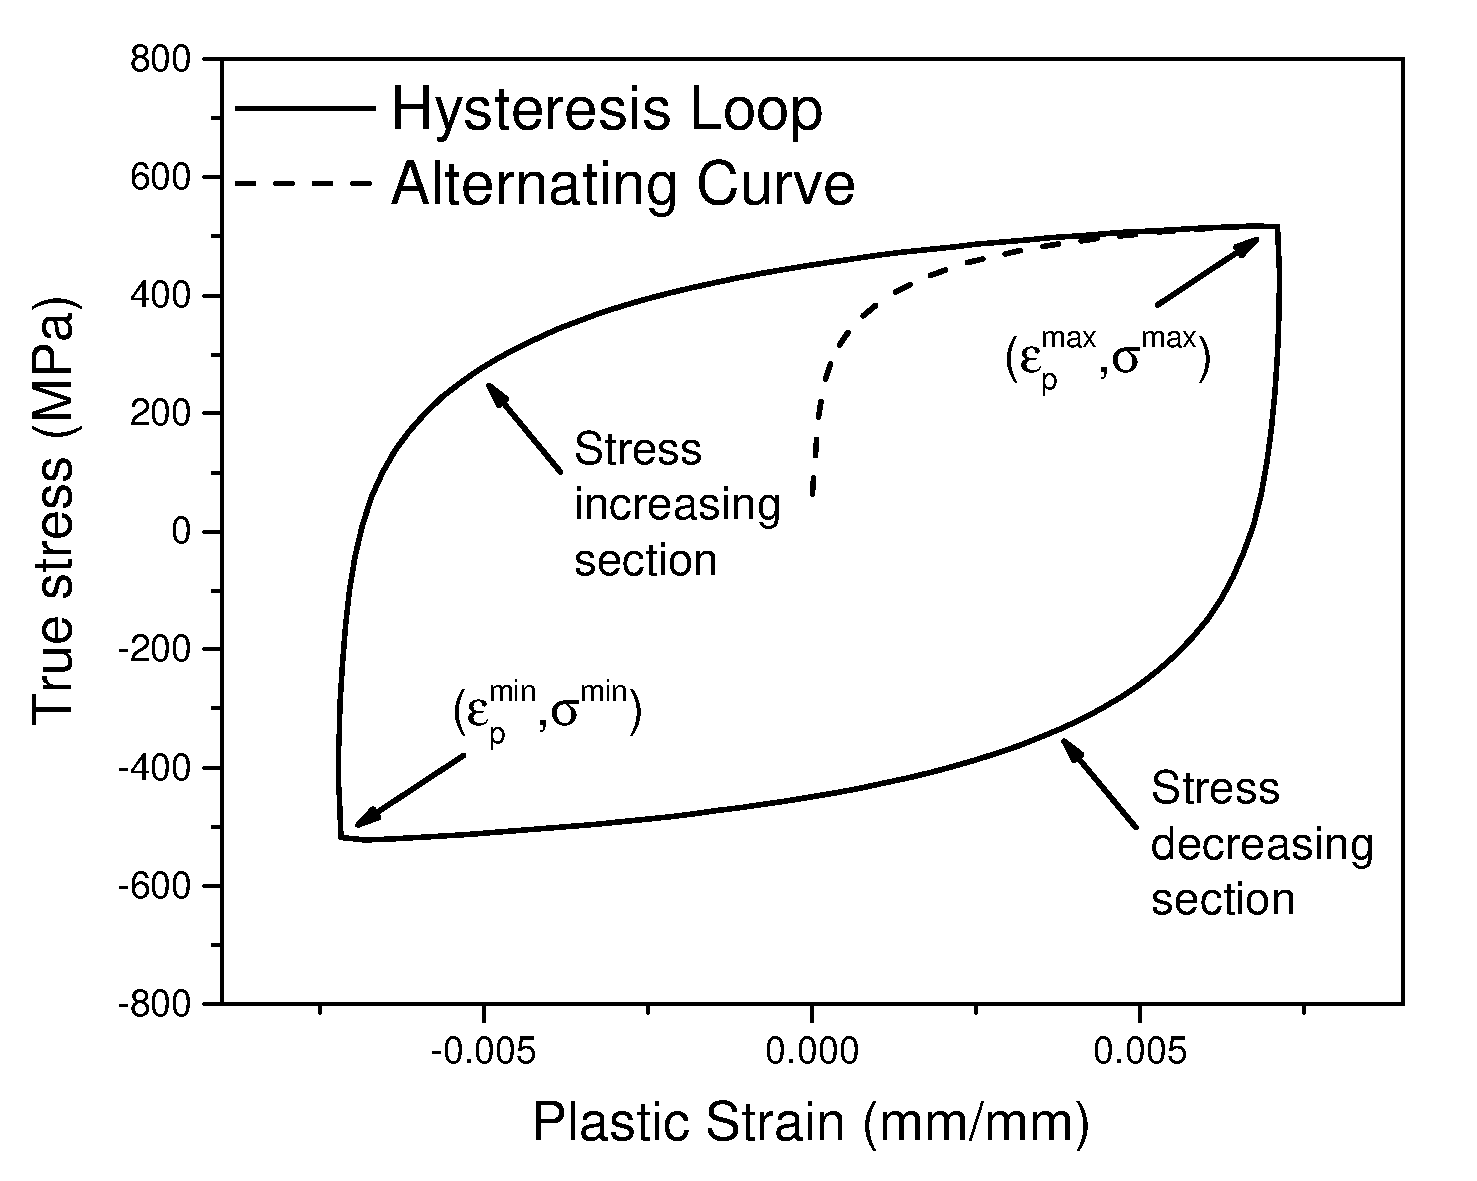
\includegraphics[width=8cm]{AlternatingCurve.pdf}
  \caption{The alternating curve is obtained from the assumed stabilized hysteresis loop.}
  \label{fig:Alternating Curve}
  \end{center}
\end{figure}


The saturated value of $c^{k}$ is denoted as $c_{s}^{k}$. Generally, when the cyclic hardening/softening is stabilized, the accumulated plastic strain is relatively large. As a result, this material constants $c_{s}^{k}$ can be determined by assuming that the accumulated plastic strain $p$ is infinitely large when the stabilized hysteresis loop is reached (\citeauthor{SunCyclic}, \citeyear{SunCyclic}). Therefore, the saturated value of $c^{k}$ is expressed as $c_{\mathrm{s}}^{k}=\lim _{\mathrm{p} \rightarrow \infty} c^{k}=c_{0}^{k}+c_{\Delta}^{k}$. The alternating stress-strain curve is divided into 4 sections at the same plastic strain point as that of the monotonic curve. The material constants $c_{s}^{k}$ is then determined by equations as below:

\begin{equation}
c_{\mathrm{s}}^{k}=\left(\frac{\sigma_{\mathrm{alt}}^{k}-\sigma_{\mathrm{alt}}^{k-1}}{\varepsilon_{\mathrm{p}}^{k}-\varepsilon_{\mathrm{p}}^{k-1}} -\frac{\sigma_{\mathrm{alt}}^{k+1}-\sigma_{\mathrm{alt}}^{k}}{\varepsilon_{\mathrm{p}}^{k+1}-\varepsilon_{\mathrm{P}}^{k}}\right) \\
\end{equation}

In order to describe the cyclic hardening in the constitutive model, parameter $c_{\Delta}^{k}$ is correlated with the accumulated plastic strain by a exponential function. Moreover, it is assumed that the cyclic hardening is totaly kinematic under proportional loadings to isolate the effects of these hardening laws. For the austenitic stainless steels, $c_{\Delta}^{k}/c_{s}^{k}$ is independent from index $k$ (\citeauthor{Fang2015Cyclic}, \citeyear{Fang2015Cyclic}). Therefore, the evolution of parameter $c_{\Delta}^{k}$ is modelled by Eq. (\ref{eq:Cyclic hardening parameter}) and the value is determined by the curve of peak stress versus accumulated plastic strain Fig. \ref{fig:Stress Amplitude Evolution}. The final values of model parameters are obtained by a trial and error method.
\begin{eqnarray}\label{eq:Cyclic hardening parameter}
1-\frac{\sigma-\sigma_{\max}}{\sigma_{\max}-\sigma_{\min }}&=&1- \exp\left ( -a^{k} p^{b^{k}} \right )\\
c_{\Delta}^{k}&=&c_{\Delta s}^{k}\left[1- \exp\left ( -a^{k} p^{b^{k}} \right ) \right]\\
c_{\Delta s}^{k}&=&c_{\mathrm{s}}^{k}-c_{0}^{k}
\end{eqnarray}
\begin{figure}[ht]
\centering
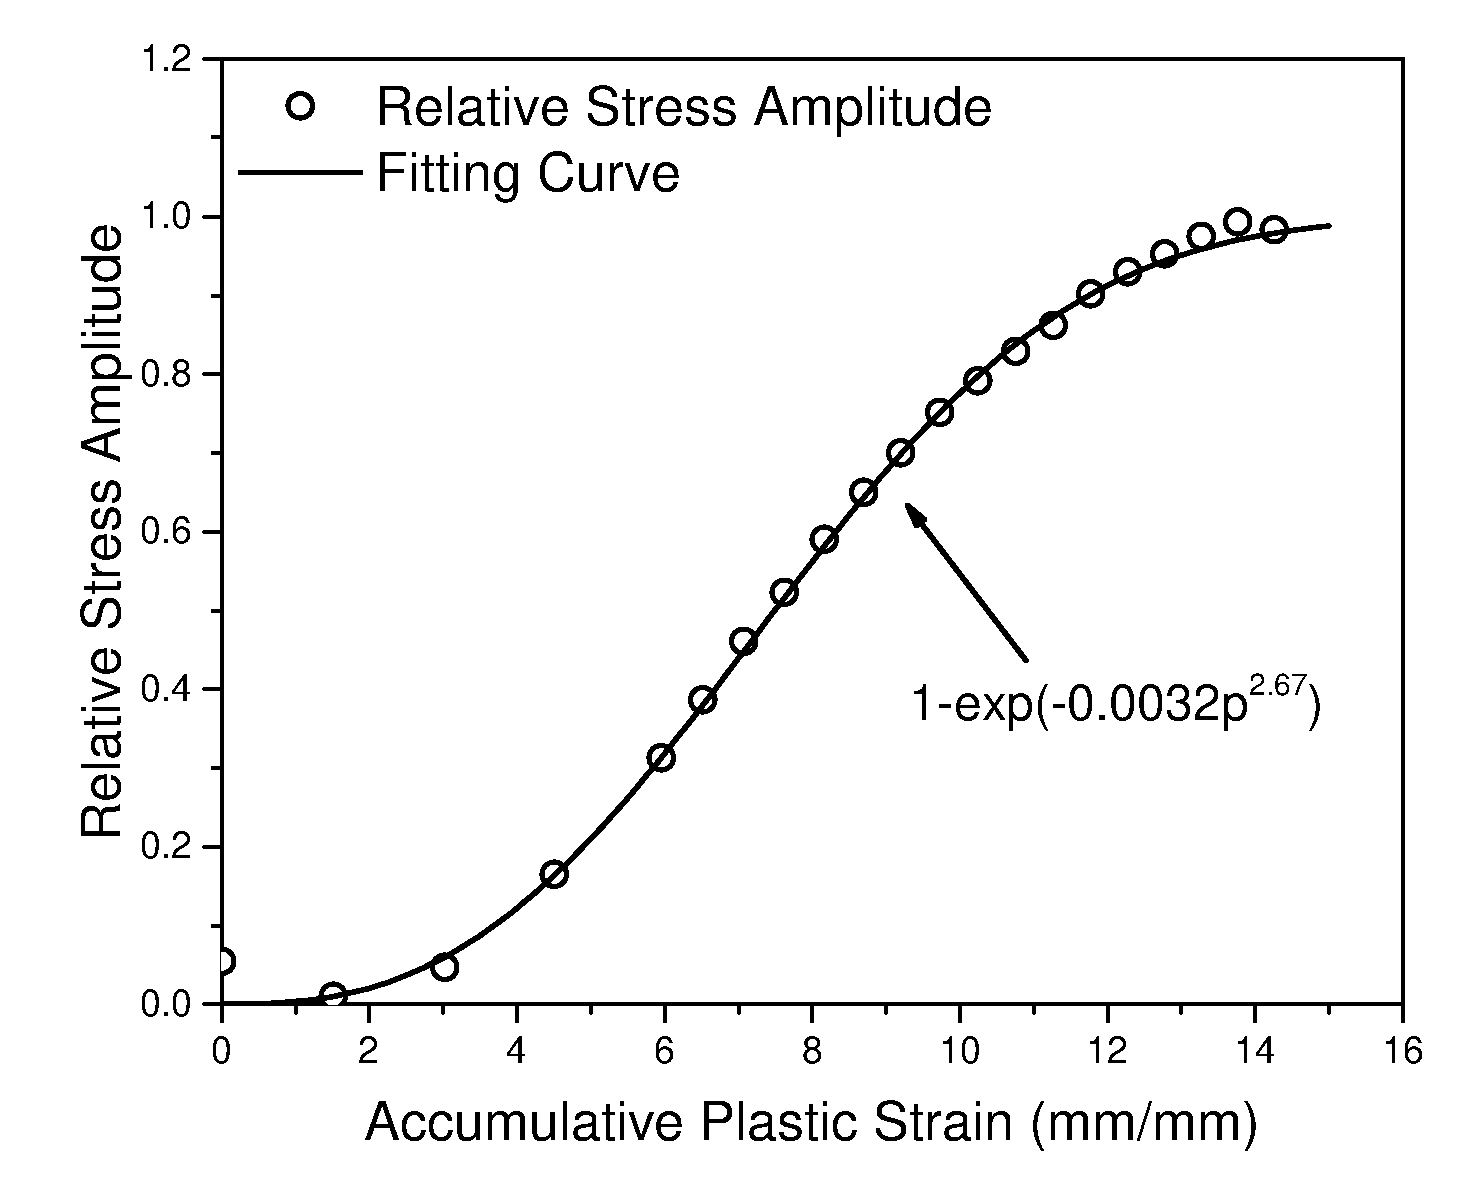
\includegraphics[width=8cm]{RelativeStressAmplitudeEvolution.pdf}
\caption{The material constants $a^{k}$ and $b^{k}$ are determined by the evolution of the relative stress amplitudes.}
\label{fig:Stress Amplitude Evolution}
\end{figure}


\begin{table*}[htbp]
\centering
\caption{Model parameters (stress unit: MPa, strain unit: mm/mm)}
\begin{tabular}{llllllllllll}
\hline
\multicolumn{2}{l}{General} & \multicolumn{2}{l}{Isotropic Hardening} & \multicolumn{4}{l}{Kinematic Hardening} & \multicolumn{4}{l}{Cyclic Hardening} \\ \hline
E               & 180000 & $y_{pt}$ & 189.0       & $c^{1}$  & 204211    & $\gamma^{1}$ & 2000      & $c_{\Delta s}^{1}$                  & 10.6 & $a^{k}$ & -0.0032 \\
$\nu$        & 0.3        &                 &                 & $c^{2}$  & 54643      & $\gamma^{2}$ & 1000      & $c_{\Delta s}^{2}$                  & 27.3 & $b^{k}$ & 2.67 \\
$Y_{0}$   & 150       &                 &                 & $c^{3}$  & 20650      & $\gamma^{3}$ & 200        & $c_{\Delta s}^{3}$                  & 108.3 \\
                 &              &                 &                 & $m^{k}$ &0.2            &                            &               &                                                   &      &              & \\ \hline
\end{tabular}
\label{tab:Model Parameters}
\end{table*}

The determined model parameters are displayed in the Table \ref{tab:Model Parameters}.
Simulation was conducted and the martensite evolution together with stress-strain response was obtained. The evolutions of peak and valley equivalent stresses during the cyclic loading tests are compared with the experimental results in Fig. \ref{fig:Comparison of PeakValleyStress}. It is reflected that the kinetics model and the cyclic plasticity model can well describe the mechanical behavior under martensitic transformation. The predicted equivalent peak and valley stresses are 10\% higher around 1000th cycle for cyclic loading tests with $\varepsilon _{\rm a}=0.5\%$. It is due to the assumption about the stabilized hysteresis loop which is proposed in the cyclic plasticity model earlier. Since the martensite contents keep rising along the number of cycles to the end of the tests, it would be more reasonable to monitor the whole evolution of peak and valley stresses instead of assuming the 260th cycle as stabilized for cyclic loading tests with $\varepsilon _{\rm a}=1.0\%$.

\begin{figure}[htbp]
  \begin{center}
  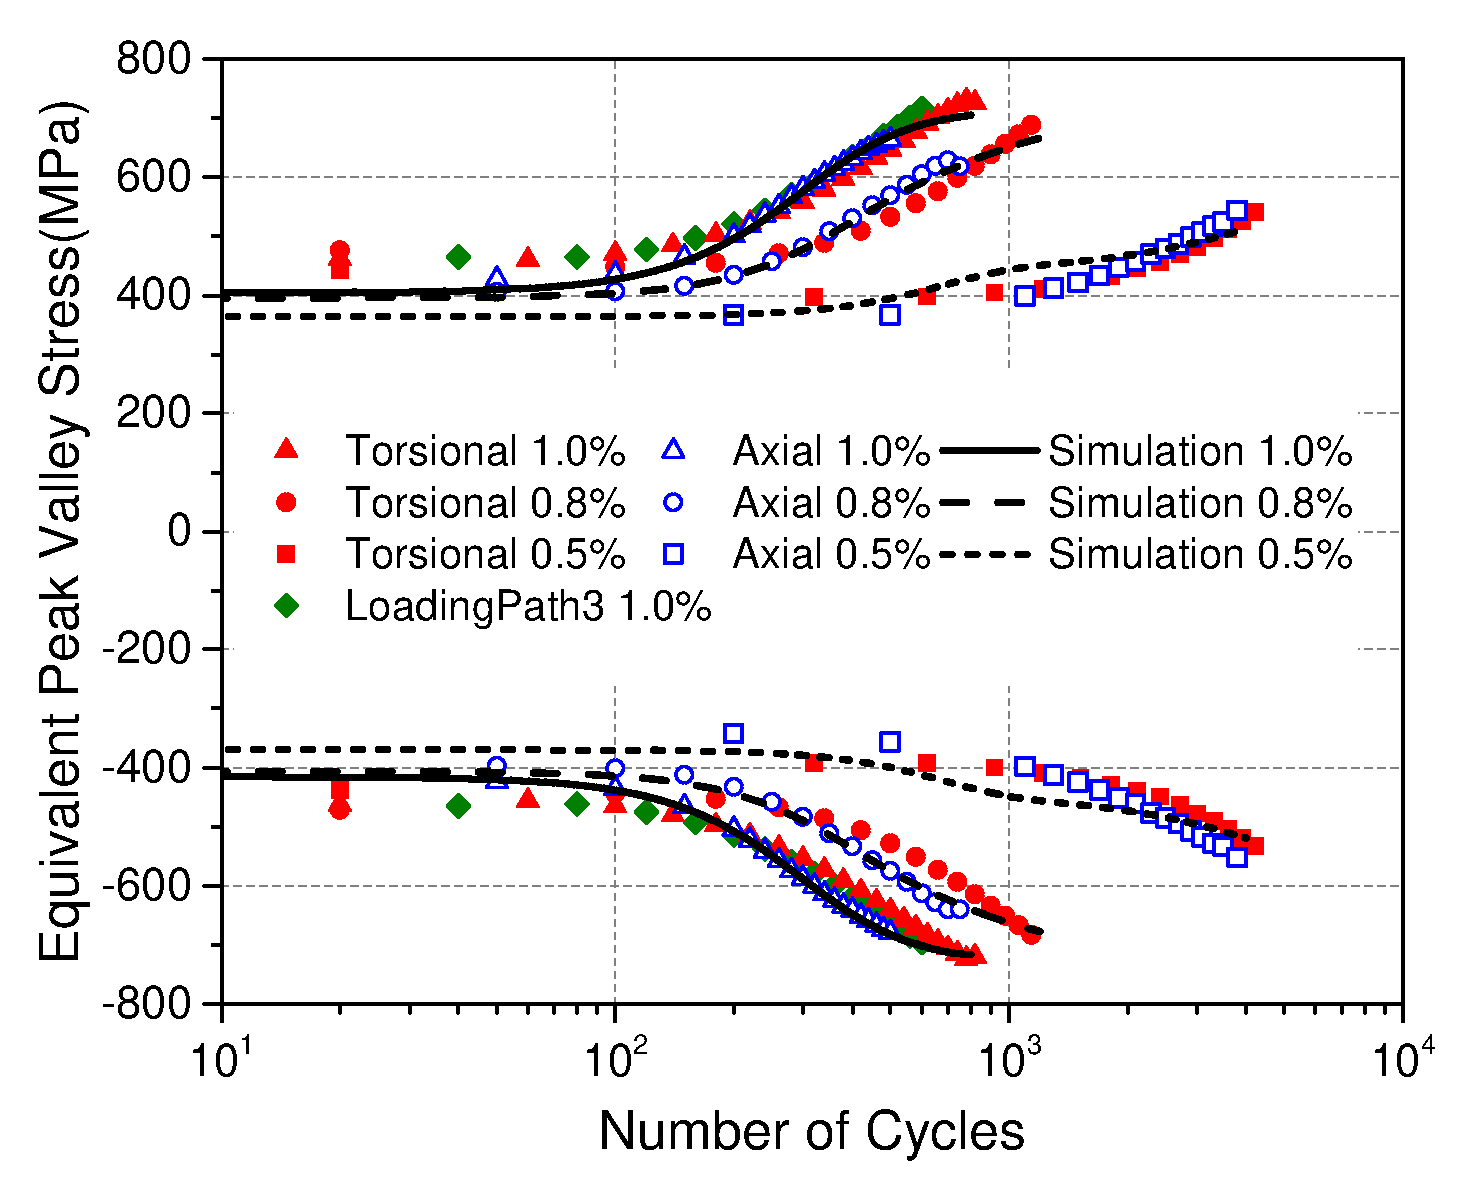
\includegraphics[width=8cm]{PeakValleyStress.pdf}
  \caption{The comparison of the peak and valley equivalent stresses predicted by simulation and experimental results.}
  \label{fig:Comparison of PeakValleyStress}
  \end{center}
\end{figure}


\begin{figure}[!ht]
\centering
\subfigure[The prediction of stress-strain response of tests with equivalent strain amplitude $\varepsilon _{\rm a}=1.0\%$]{
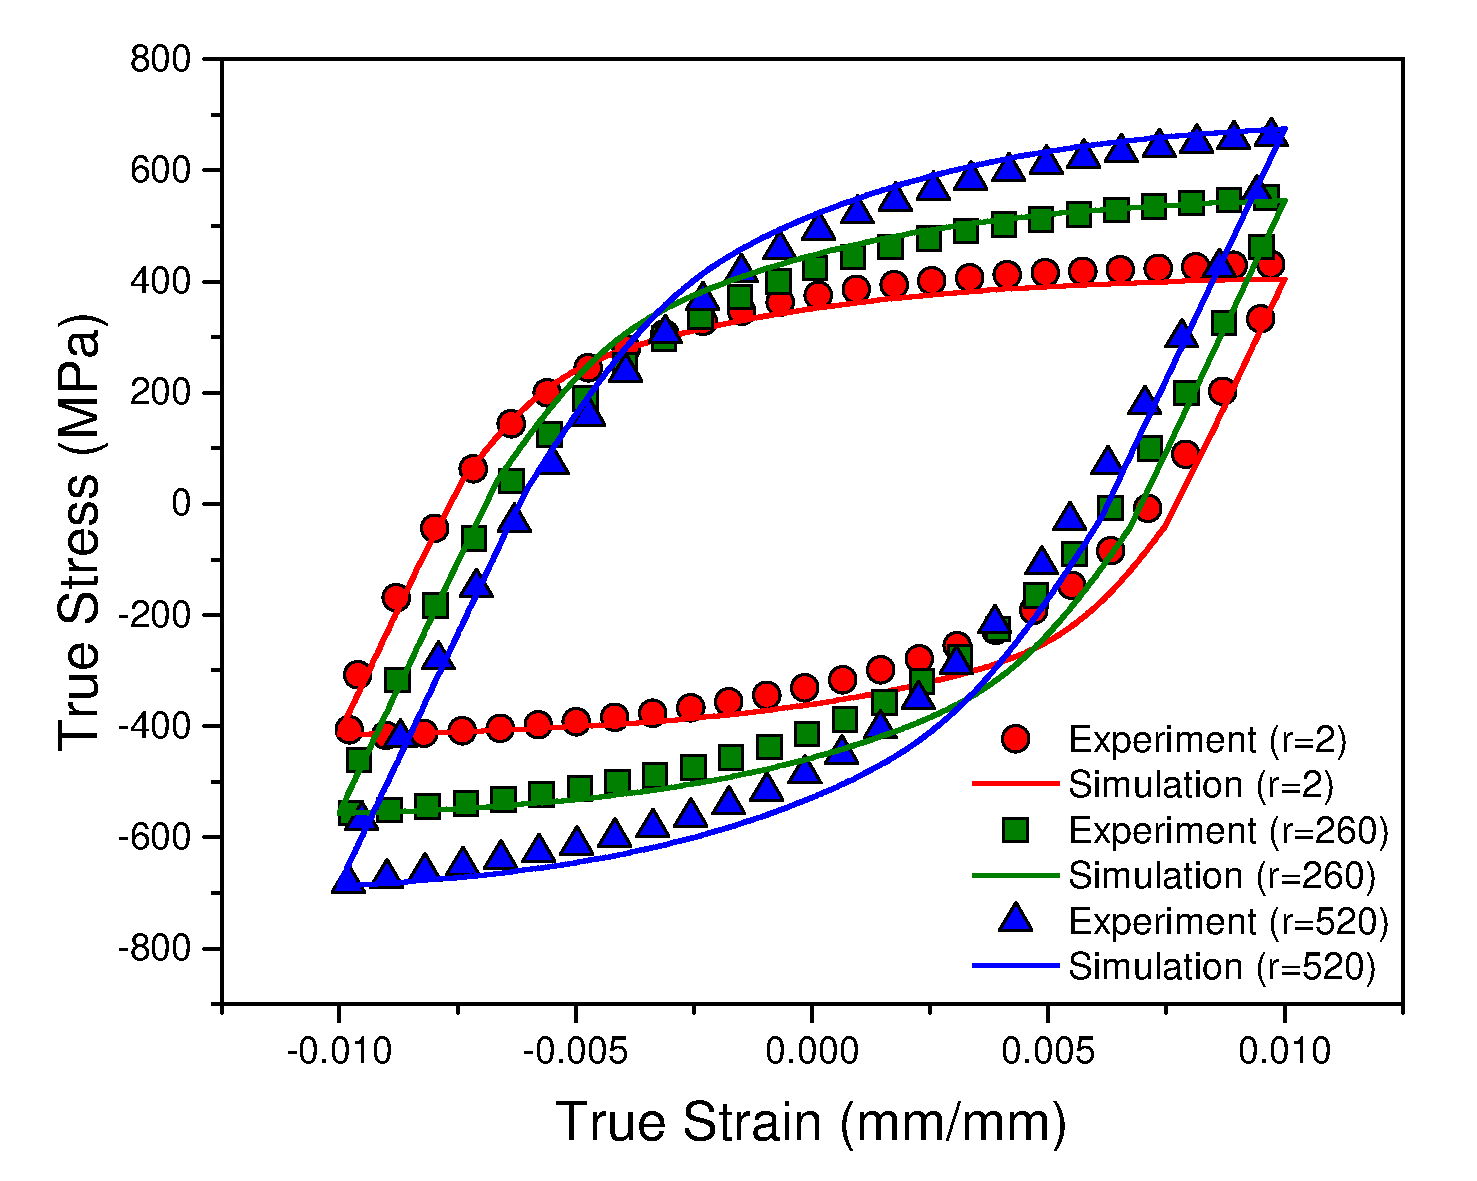
\includegraphics[width=8cm]{ComparisonStrain10.pdf}
}
\quad
\subfigure[The prediction of stress-strain response of tests with equivalent strain amplitude $\varepsilon _{\rm a}=0.8\%$]{
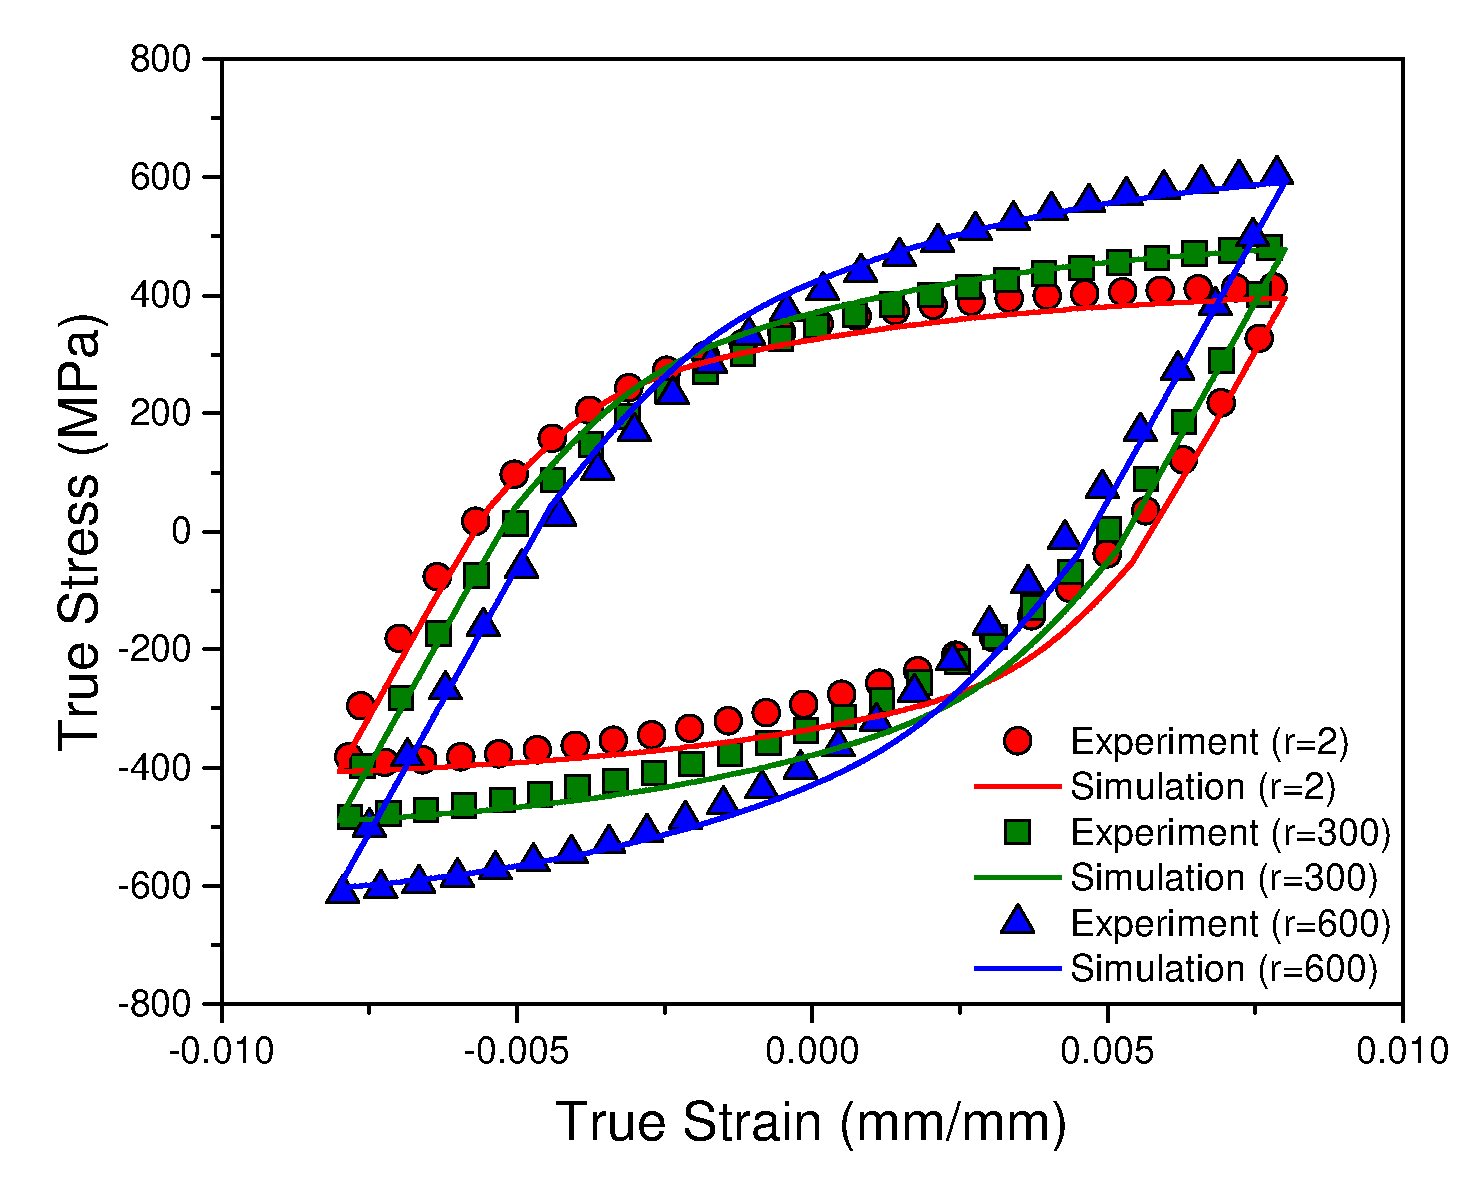
\includegraphics[width=8cm]{ComparisonStrain08.pdf}
}
\quad
\subfigure[The prediction of stress-strain response of tests with equivalent strain amplitude $\varepsilon _{\rm a}=0.5\%$]{
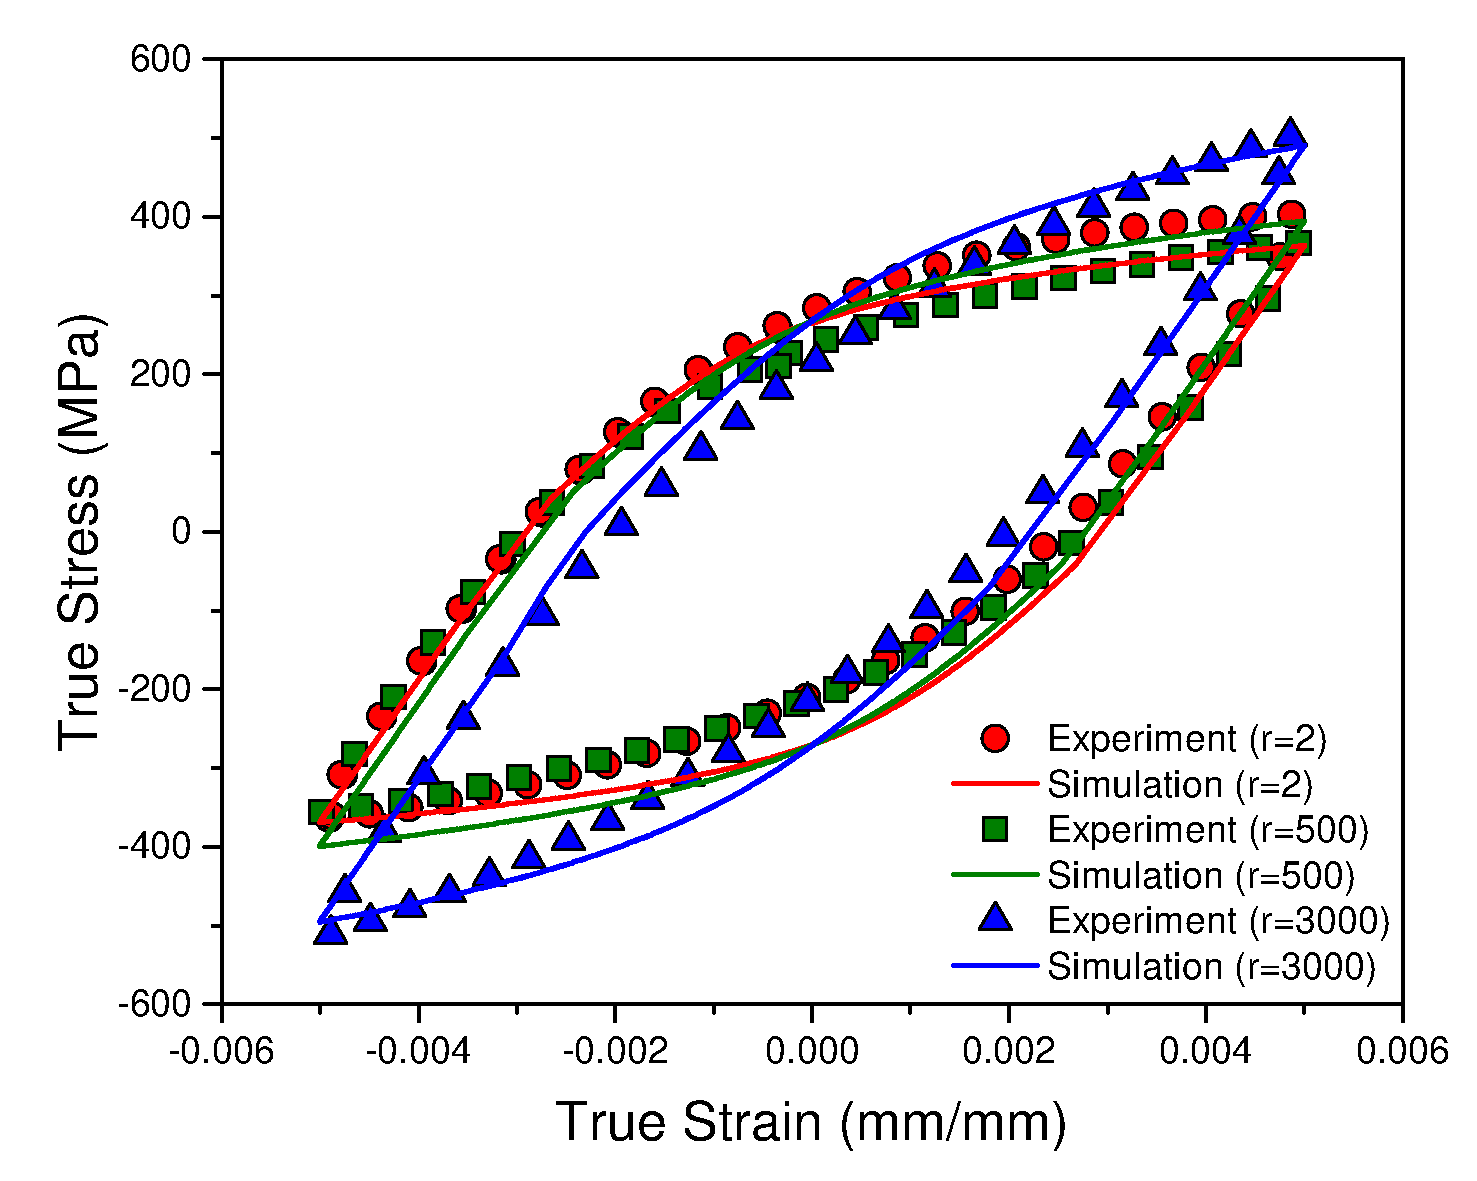
\includegraphics[width=8cm]{ComparisonStrain05.pdf}
}
\caption{The comparison of the stress-strain curve predicted by simulation and experimental results}
\label{fig:Comparison of Strain10}
\end{figure}



%\begin{figure}[htbp]
%  \begin{center}
%  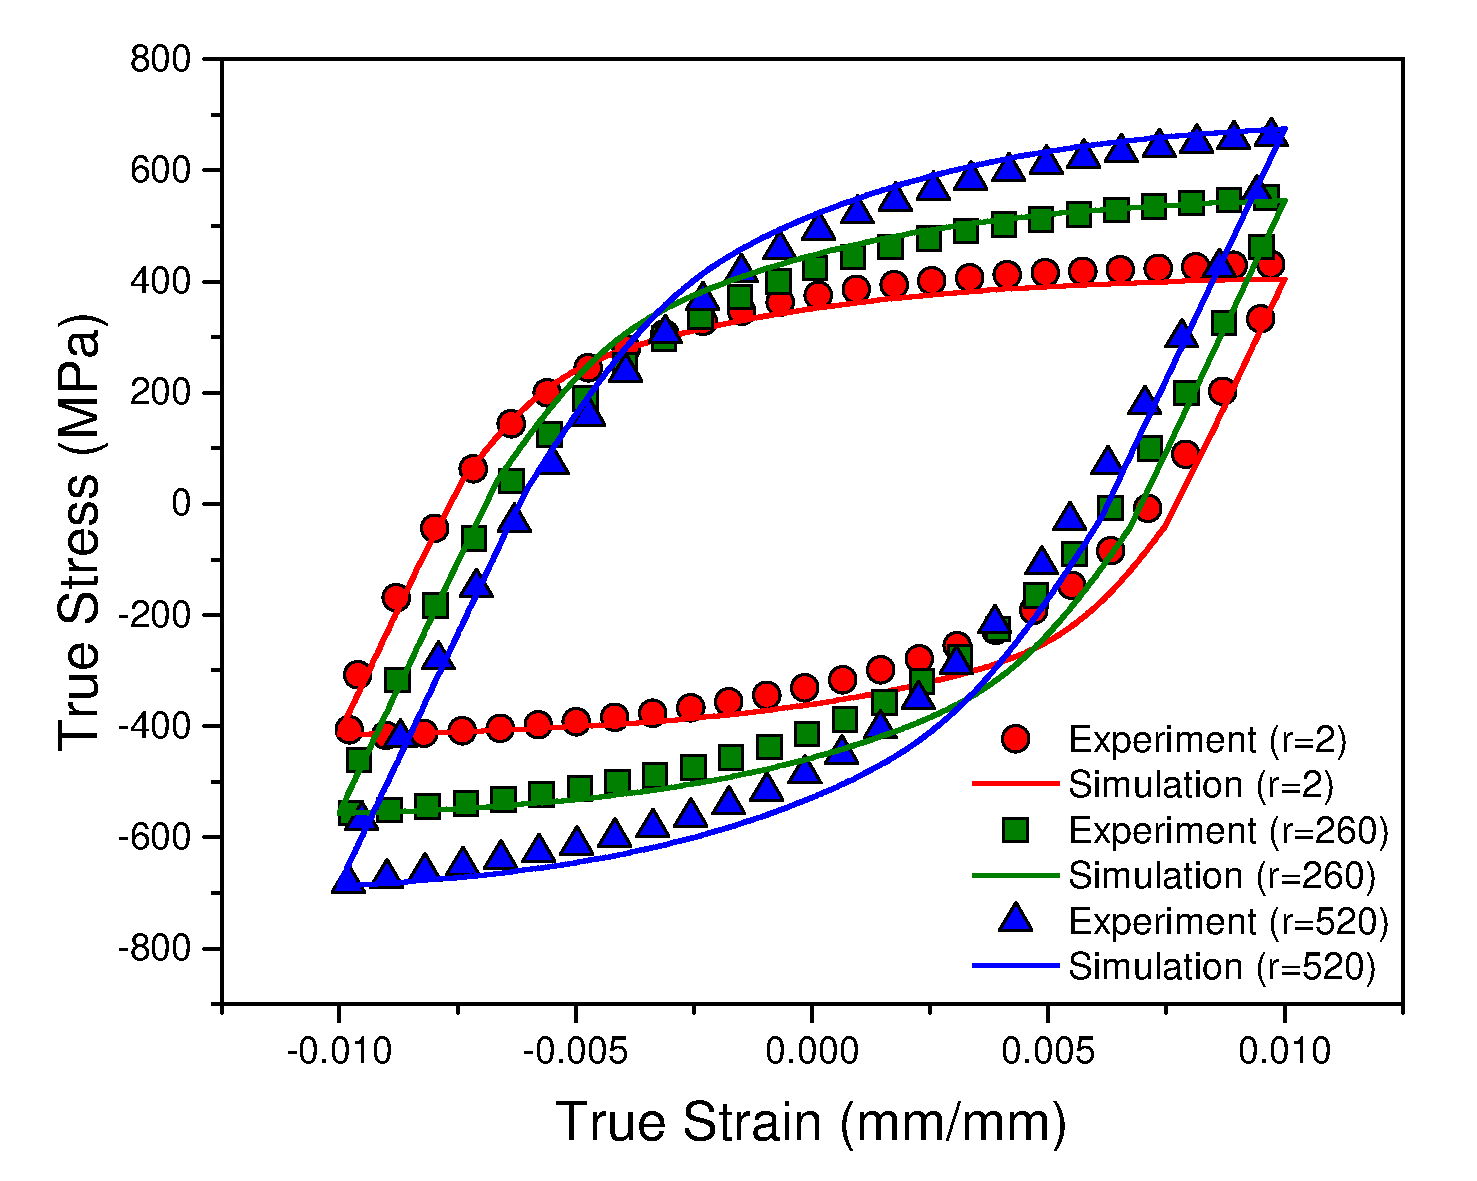
\includegraphics[width=8cm]{ComparisonStrain10.pdf}
%  \caption{The comparison of the stress-strain curve predicted by simulation and experimental results}
%  \label{fig:Comparison of Strain10}
%  \end{center}
%\end{figure}
%
%\begin{figure}[htbp]
%  \begin{center}
%  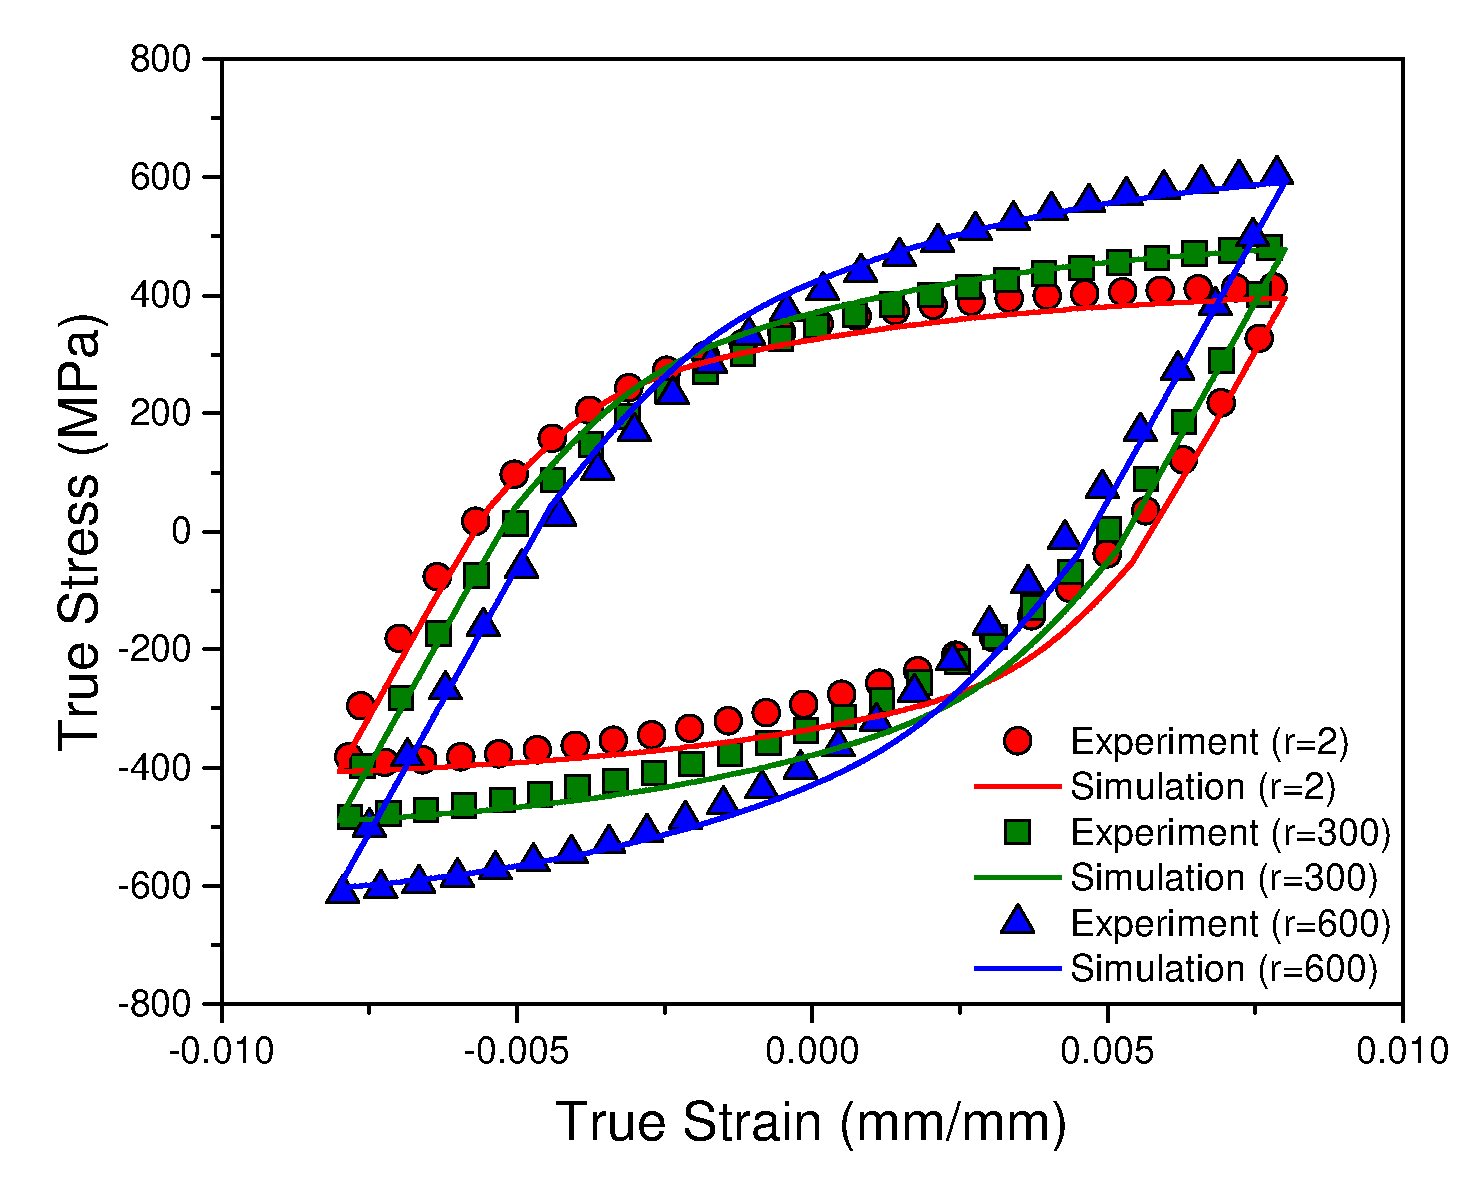
\includegraphics[width=8cm]{ComparisonStrain08.pdf}
%  \caption{The comparison of the stress-strain curve predicted by simulation and experimental results}
%  \label{fig:Comparison of Strain08}
%  \end{center}
%\end{figure}
%
%\begin{figure}[htbp]
%  \begin{center}
%  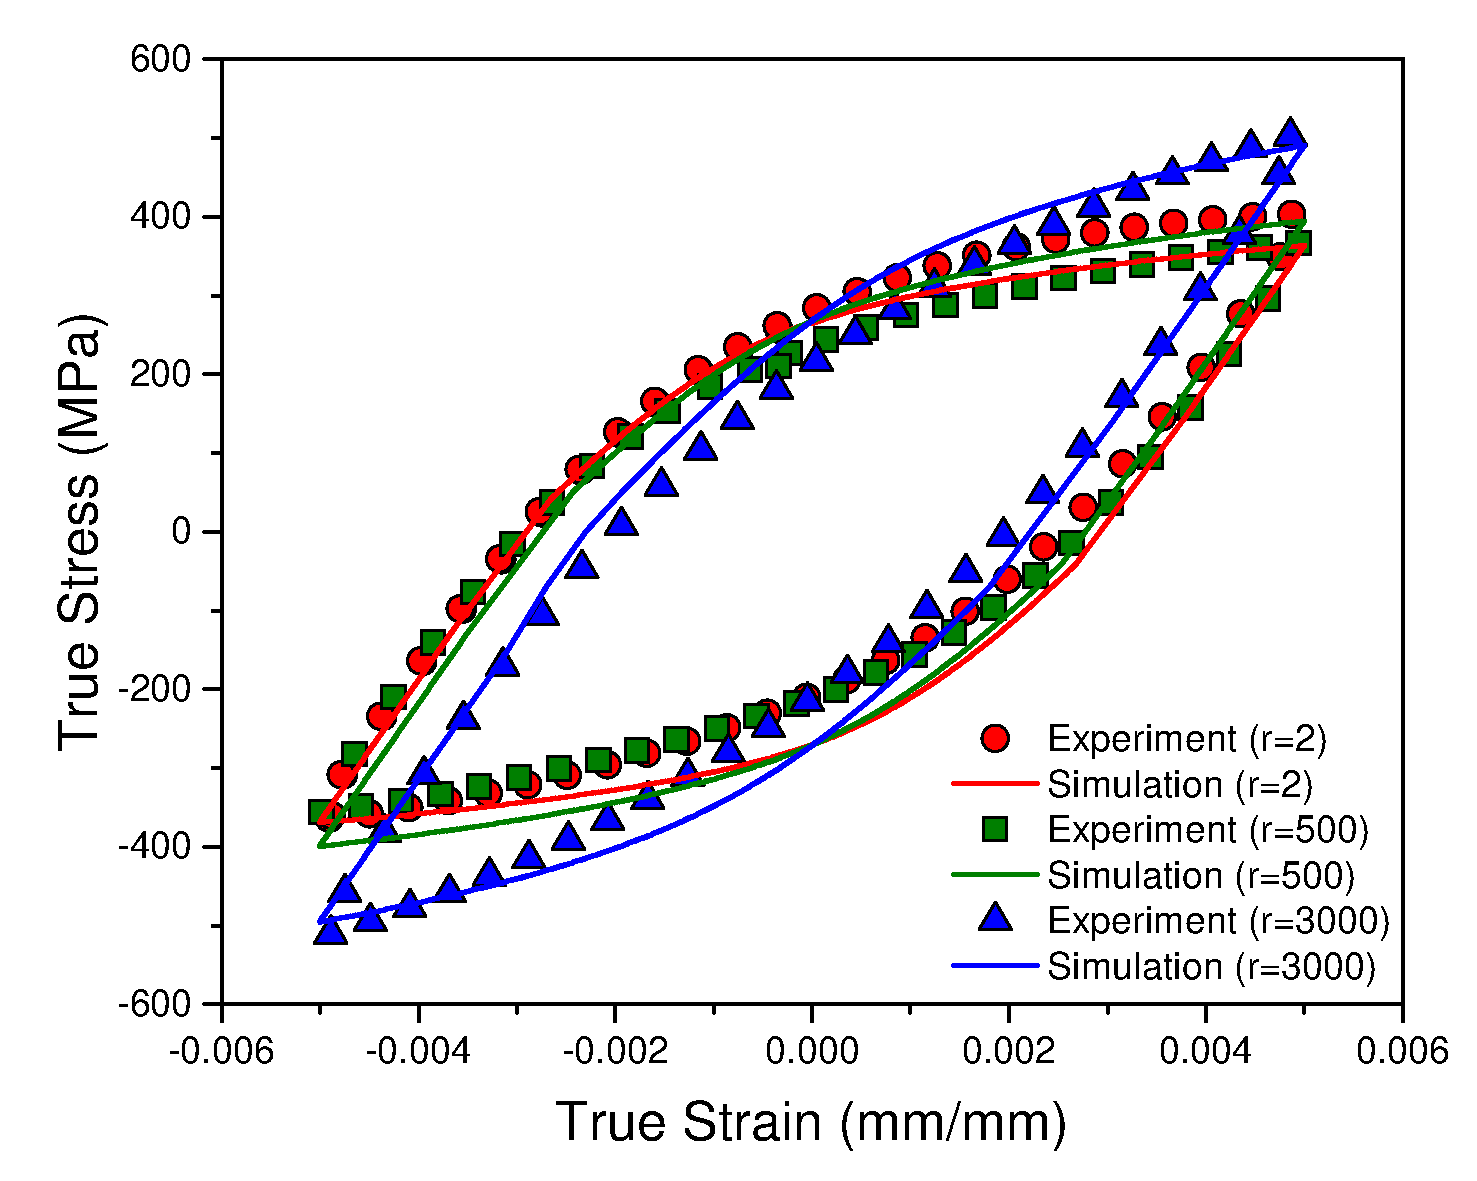
\includegraphics[width=8cm]{ComparisonStrain05.pdf}
%  \caption{The comparison of the stress-strain curve predicted by simulation and experimental results}
%  \label{fig:Comparison of Strain05}
%  \end{center}
%\end{figure}

In order to verify the constitutive model of AISI 348 considering martensitic transformation, stress-strain curves of certain cycles of the experiments were chosen for comparison with the simulation results. For axial cyclic loading tests with a strain amplitude $\varepsilon _{\rm a}=1.0\%$, the second cycle with a martensite content of $\chi=0$, the 260th cycle with a martensite content of $\chi=0.3995$ and the 520th cycle with a martensite content of $\chi=0.8620$ were selected. For axial cyclic loading tests with a strain amplitude $\varepsilon _{\rm a}=0.8\%$, the second cycle with a martensite content of $\chi=0$, the 300th cycle with a martensite content of $\chi=0.2210$ and the 600th cycle with a martensite content of $\chi=0.6531$ were selected. For axial cyclic loading tests with a strain amplitude $\varepsilon _{\rm a}=0.5\%$, the second cycle with a martensite content of $\chi=0$, the 500th cycle with a martensite content of $\chi=0.0269$ and the 3000th cycle with a martensite content of $\chi=0.3381$ were selected.

The comparison of the stress-strain curve predicted by simulation and experimental results is shown in Fig. \ref{fig:Comparison of Strain10}. It can be drawn from the figure that the cyclic plasticity model can well describe the stress-strain response during most part of the whole process. However, it can be observed from the comparison of cyclic loading tests with $\varepsilon _{\rm a}=0.5\%$ that the value of stress is slightly underestimated for the 500th cycle. This is due to the neglecting of cyclic softening at the early stage of the cyclic loading tests.

%\begin{figure*}[ht]
%\centering
%\includegraphics[width=5cm]{Strain10r=1.pdf}
%\label{fig_framework}
%\end{figure*}

%\begin{figure*}[htbpt]
%\centering
%\subfigure[Axial 1.0$\%$ 1st cycle $\chi=0$]{
%\includegraphics[width=5cm]{Strain10r=1.pdf}
%}
%\subfigure[Axial 1.0$\%$ 260th cycle $\chi=0.2357$]{
%\includegraphics[width=5cm]{Strain10r=260.pdf}
%}
%\subfigure[Axial 1.0$\%$ 520th cycle $\chi=0.5086$]{
%\includegraphics[width=5cm]{Strain10r=520.pdf}
%}
%\subfigure[Axial 0.8$\%$ 1st cycle $\chi=0$]{
%\includegraphics[width=5cm]{Strain08r=1.pdf}
%}
%\subfigure[Axial 0.8$\%$ 300th cycle $\chi=0.1304$]{
%\includegraphics[width=5cm]{Strain08r=300.pdf}
%}
%\subfigure[Axial 0.8$\%$ 600th cycle $\chi=0.3853$]{
%\includegraphics[width=5cm]{Strain08r=600.pdf}
%}
%\subfigure[Axial 0.5$\%$ 1st cycle $\chi=0$]{
%\includegraphics[width=5cm]{Strain05r=1.pdf}
%}
%\subfigure[Axial 0.5$\%$ 500th cycle $\chi=0.0159$]{
%\includegraphics[width=5cm]{Strain05r=500.pdf}
%}
%\subfigure[Axial 0.5$\%$ 1000th cycle $\chi=0.0412$]{
%\includegraphics[width=5cm]{Strain05r=1000.pdf}
%}
%\caption{The prediction of the model and the test hysteresis loops}
%\label{fig:Predictions}
%\end{figure*}

%The rise of the equivalent stress amplitudes along the martensitic transformation is well demonstrated by the model which is shown in Fig\ref{fig:Prediction of the equivalent stress amplitudes}. The maximum relative error for the prediction of the equivalent stress amplitudes does not exceed $3\%$ for the tests with strain amplitudes of $\varepsilon _{a}=0.8\%$ and $\varepsilon _{a}=1.0\%$. However, the prediction for the tests with strain amplitudes of $\varepsilon _{a}=0.5\%$ was insufficiently accurate (the maximum relative error reached 10$\%$) and it was due to the error of the prediction of martensite content.
%
%\begin{figure}[htbp]
%  \begin{center}
%  \includegraphics[width=8cm]{PredictionofStressAmplitudes.pdf}
%  \caption{The prediction of the equivalent stress amplitudes by the model}
%  \label{fig:Prediction of the equivalent stress amplitudes}
%  \end{center}
%\end{figure}

\section{Conclusions}

The martensitic transformation under multi-axial proportional cyclic loadings in metastable austenitic stainless steel AISI 348 was investigated. The material exhibited initial cyclic softening and significant secondary cyclic hardening due to the growth of martensite.

The variation of martensite content within a loading cycle was observed.  It was found that the martensite content would decrease when the product of stress and strain $\sigma \cdot \varepsilon$ was greater than zero and would increase otherwise during cyclic loadings. In addition, the relative amplitude of this 'fluctuation' of martensite content and the $\varepsilon _{a}$ were positively correlated.

The evolution of the martensite content was described as a function of the accumulated equivalent plastic strain and a threshold value of equivalent plastic strain to trigger the transformation. The effect of strain amplitude was taken into account in the kinetics model. The kinetics model could degenerate into a more simplified expression to describe the martensitic transformation under monotonic loadings. The martensite content calculated on the basis of this kinetics model was in excellent accordance with the experimentally obtained data.

A cyclic plasticity model for AISI 348 was established by correlating the isotropic hardening and the effect of martensitic transformation. The secondary hardening behavior of the material was well described and the equivalent peak and valley stresses predicted by the model matched well with the experimental results.

Future work will expand the model to describe the mechanical behavior of AISI 348 under non-proportional loading paths. The cyclic softening will be taken into account in the cyclic plasticity model. In addition, the change of martensite content within a cycle will be considered for a more accurate transformation kinetics model.


\section*{Acknowledgment:} The present work is financed by the China Natural Science Foundation under the contract numbers 11572169 and 51775294.

\section*{References}

%\bibliographystyle{unsrt}            % bibliography style
%\bibliographystyle{elsarticle-num}
%\bibliographystyle{model4-names}
\bibliographystyle{elsarticle-harv}
\biboptions{authoryear}
% \bibliographystyle{plain}            % bibliography style
% \bibliography{bibliography}          % personal bibliography file
\bibliography{mybibfile}

\end{document} 